\documentclass{beamer}
\usepackage[utf8]{inputenc}
\usepackage{amsmath, amssymb, bm}
\usepackage{physics}
\usepackage{graphicx}
\usepackage{hyperref}
\usepackage{xmpmulti}
\usepackage{tikz}
\usetheme{Madrid} % You can change the theme as you like
\usecolortheme{seagull}


\begin{document}

\title[Quantum Computing and ML]{\textbf{Quantum Technology and Artificial Intelligence}}
\author{Morten Hjorth-Jensen, mhjensen@uio.no}
\institute{Department of Physics and Center for Computing in Science Education, University of Oslo, Norway}
\date{August 14, 2025}


%-----------------------------------------------------------
%\begin{frame}
%    \titlepage
%\end{frame}

%-----------------------------------------------------------


\begin{frame}[plain,fragile]
\titlepage
\end{frame}

\begin{frame}[plain,fragile]
\frametitle{What is this talk about?}

\begin{block}{}
The main emphasis is to give you a short and hopefully pedestrian overview  to the whys and hows of machine learning and quantum technologies, why this could (or should) be of interest and where to find info about courses and study programs at UiO. 
\end{block}

\end{frame}


\begin{frame}[plain,fragile]
\frametitle{Multiscale scientific problem, life science example}


% inline figure
\centerline{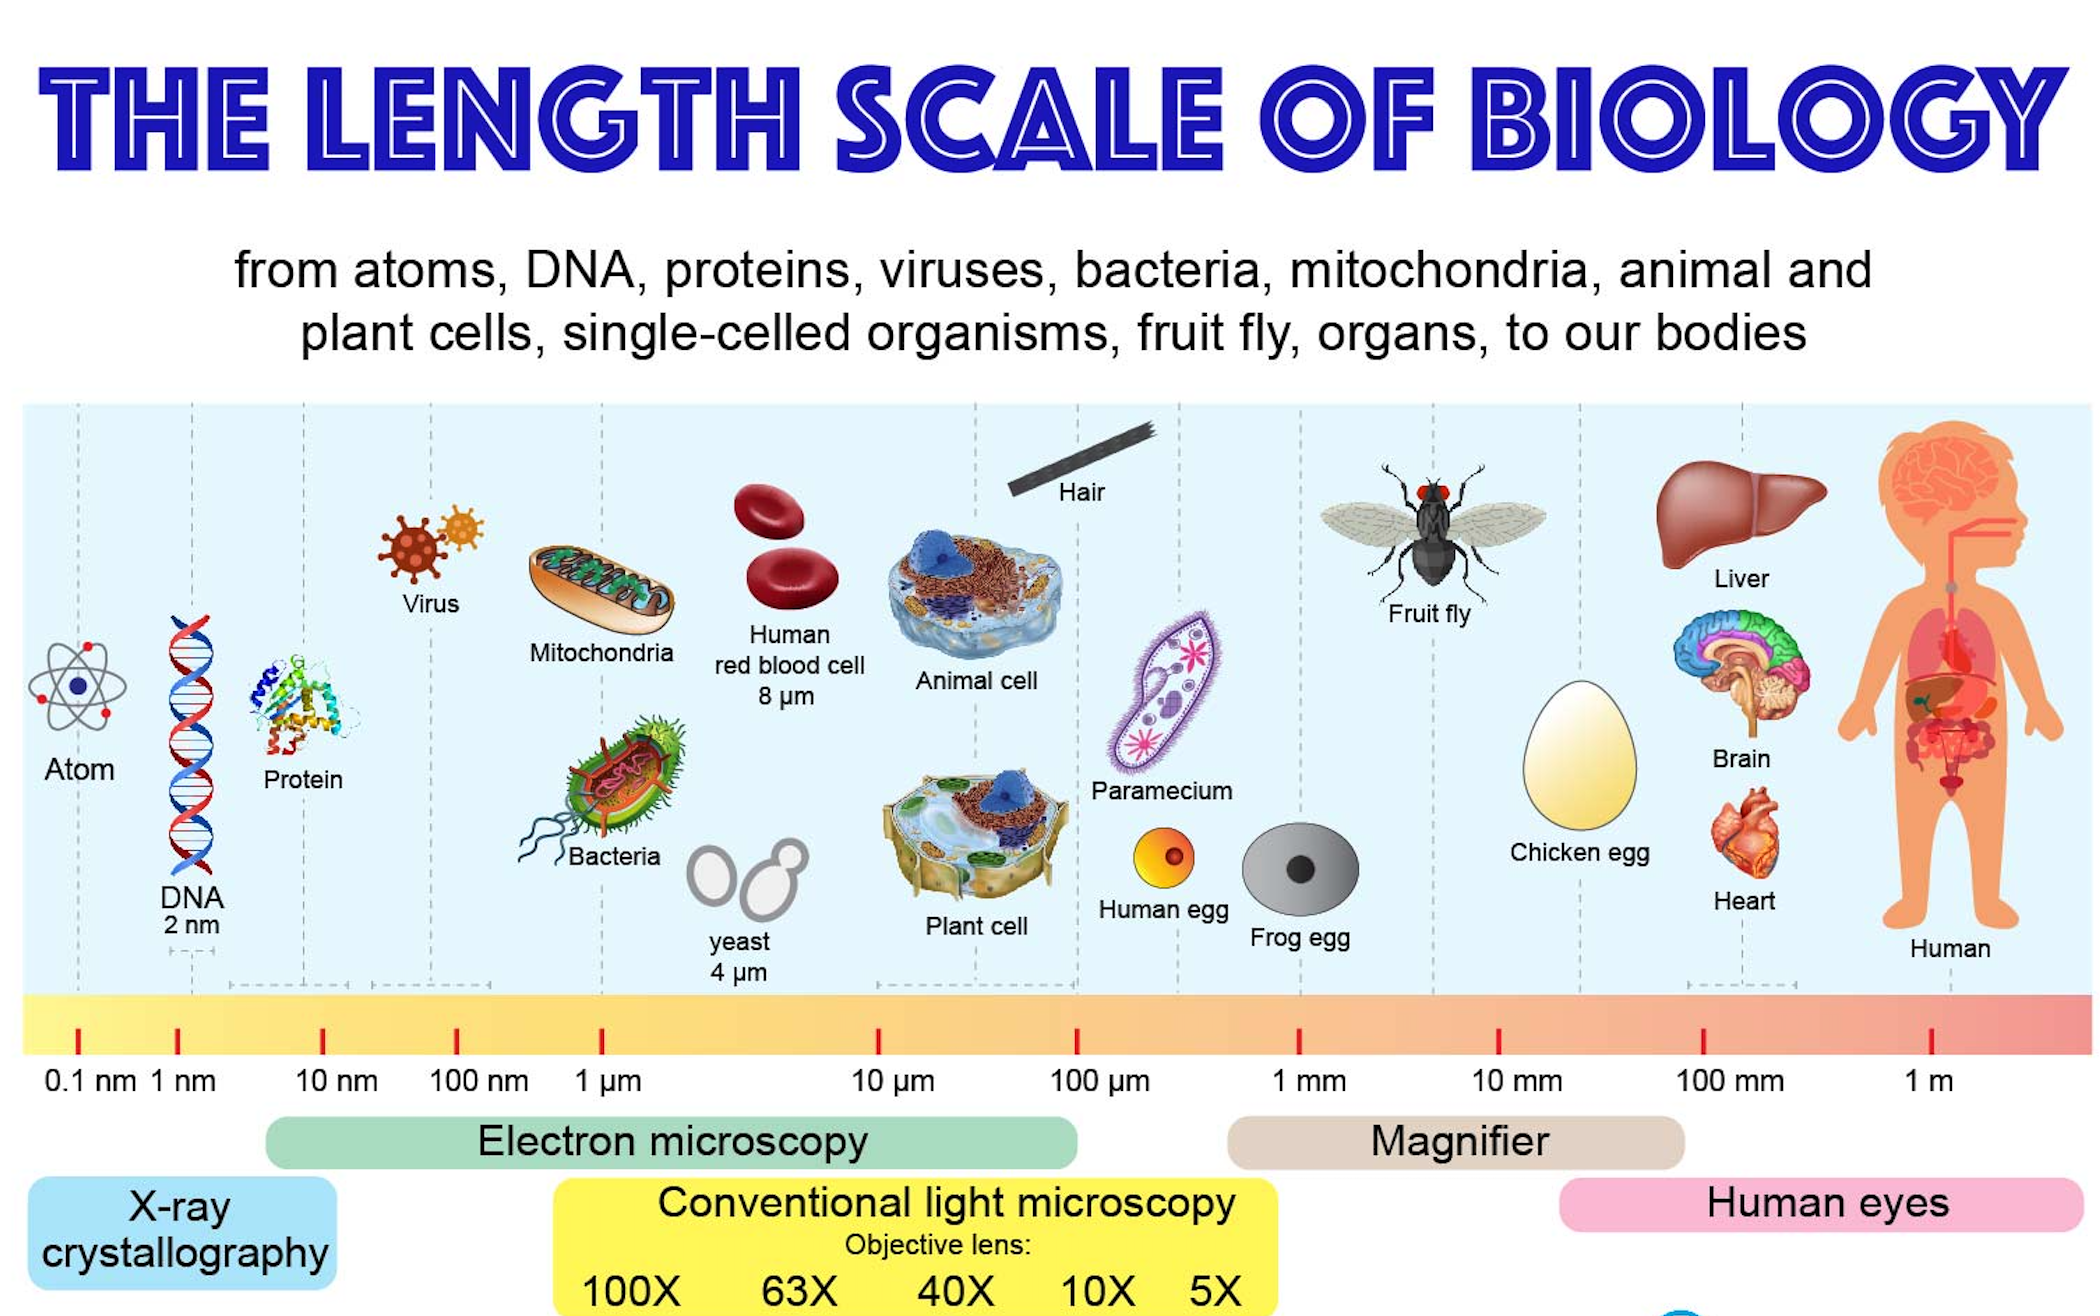
\includegraphics[width=1.05\linewidth]{figures/science2.png}}

\end{frame}


\begin{frame}[plain,fragile]
\frametitle{Multiscale scientific problem, life science example, with mathematical methods}


% inline figure
\centerline{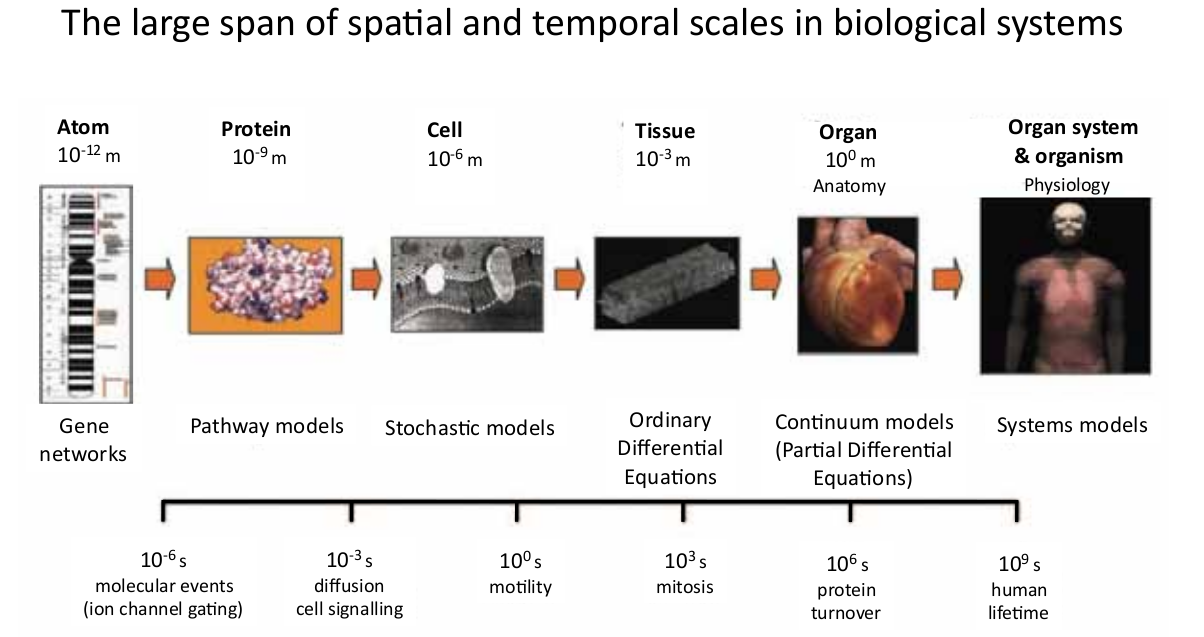
\includegraphics[width=1.05\linewidth]{figures/science1.png}}

\end{frame}


\begin{frame}[plain,fragile]
\frametitle{Multiscale scientific problem, life science example with Machine learning}


% inline figure
\centerline{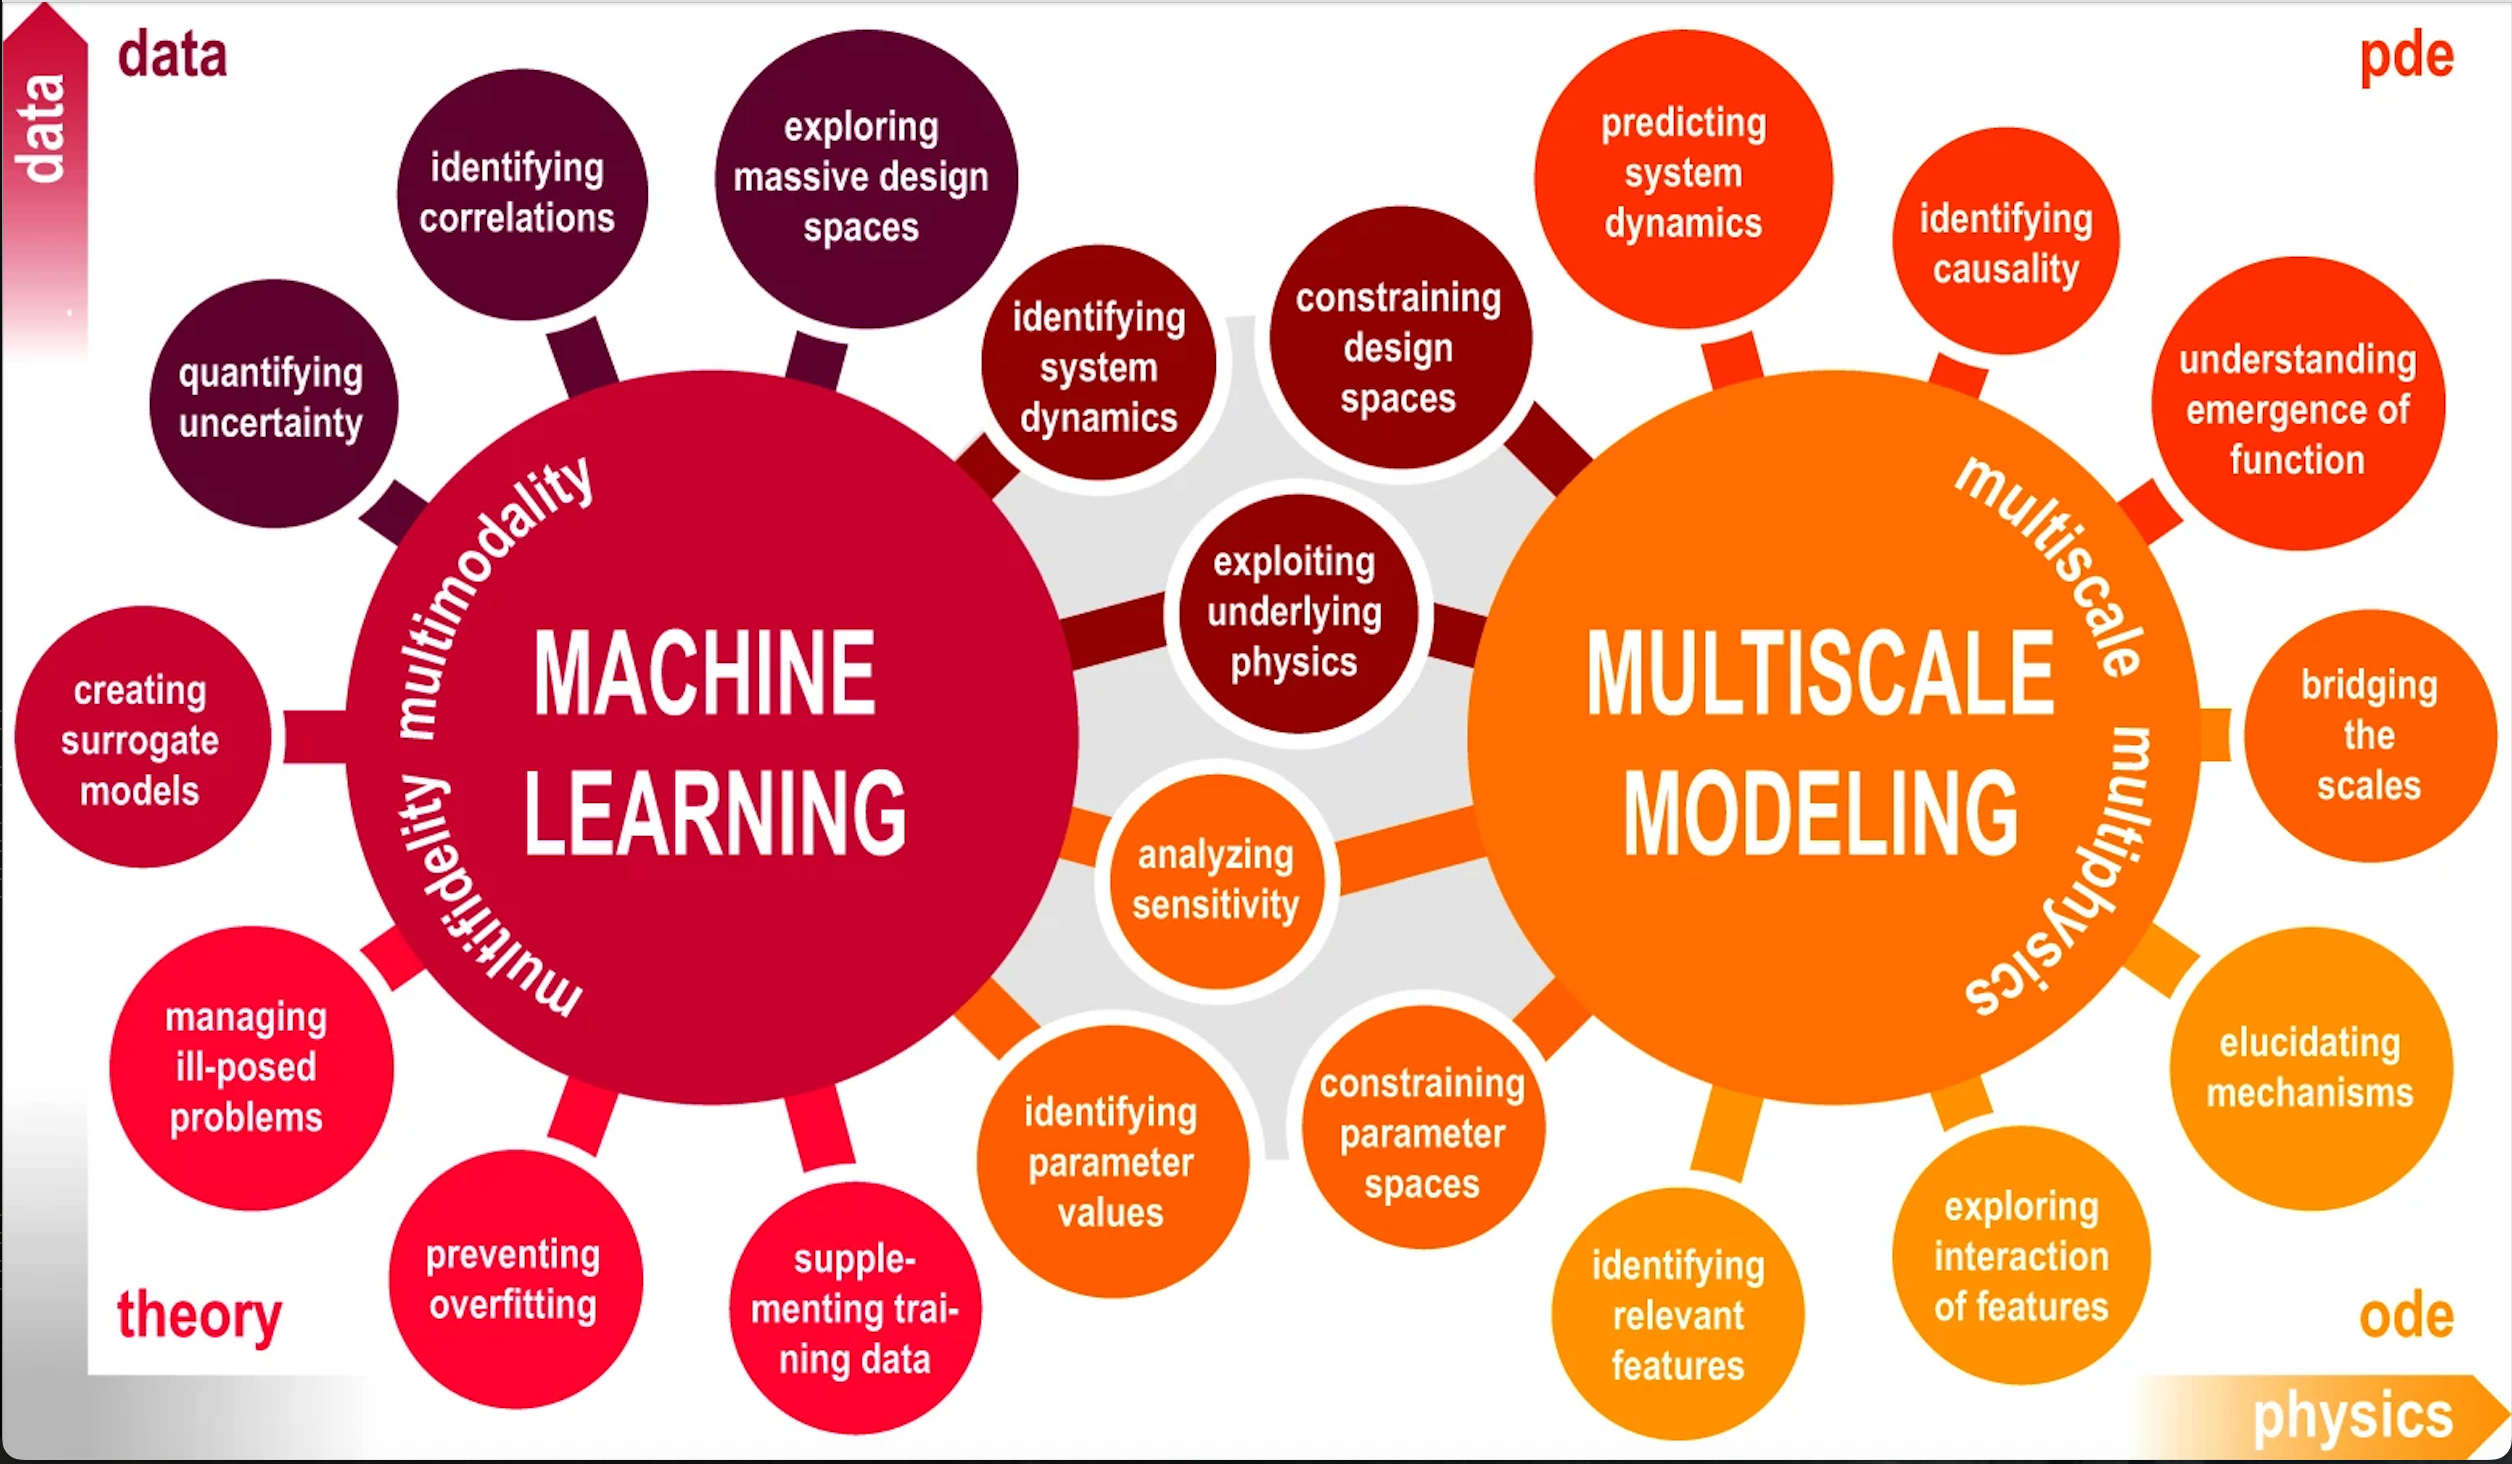
\includegraphics[width=1.05\linewidth]{figures/science3.png}}

\end{frame}



\begin{frame}[plain,fragile]
\frametitle{Quantum technology and machine learning/AI}


% inline figure
\centerline{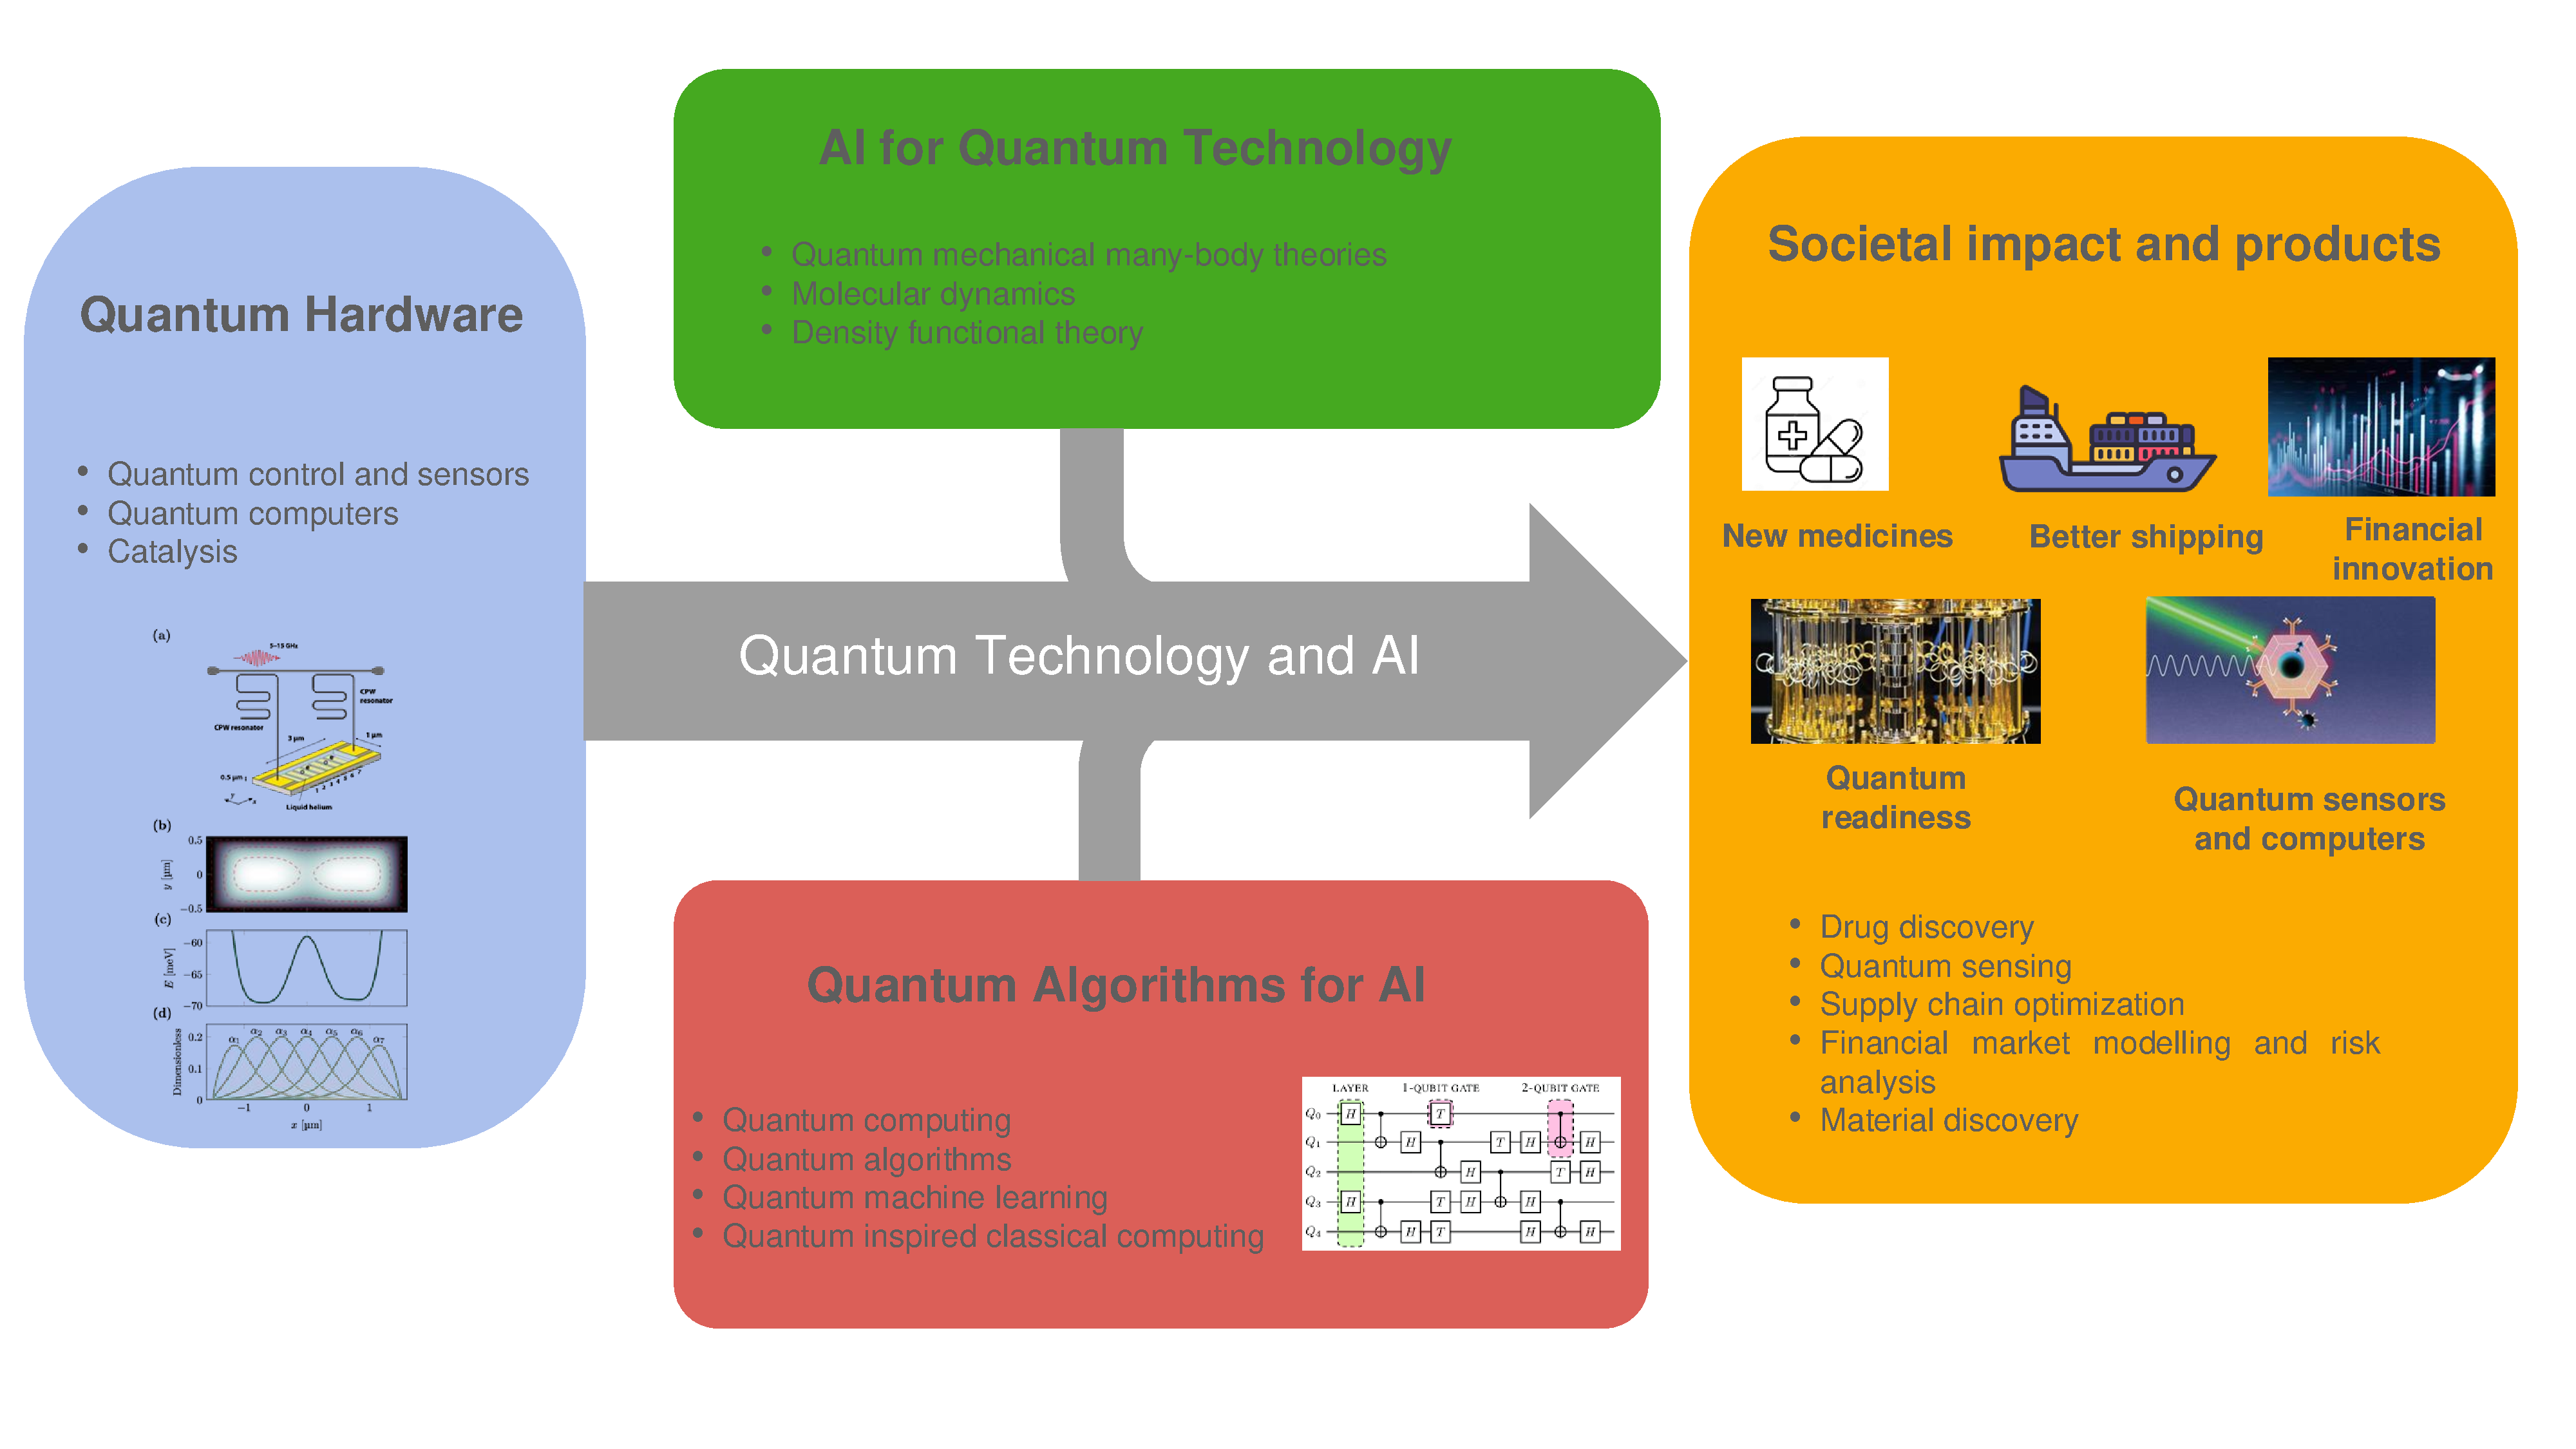
\includegraphics[width=1.05\linewidth]{figures/figureintro.pdf}}

\end{frame}



%-----------------------------------------------------------
\section{Introduction to Machine Learning}
\begin{frame}{What is Machine Learning?}
Machine Learning (ML) is the study of algorithms that improve through data experience.

\textbf{Types of Machine Learning:}
\begin{itemize}
    \item \textbf{Supervised Learning:} Labeled data for classification or regression.
    \item \textbf{Unsupervised Learning:} No labels; discover hidden patterns.
    \item \textbf{Reinforcement Learning:} Learning through interaction with the environment.
\end{itemize}


\textbf{ML Workflow:}
\[
\text{Data} \rightarrow \text{Model Training} \rightarrow \text{Prediction}
\]
\end{frame}



%-----------------------------------------------------------
\section{Introduction to Quantum Computing}
\begin{frame}{What is Quantum Computing?}
Quantum computing leverages principles of quantum mechanics to perform computations beyond classical capabilities.

\vspace{10pt}
\textbf{Key Concepts:}
\begin{itemize}
\item \textbf{Superposition:} Qubits can exist in a combination of states.
\item \textbf{Entanglement:} Correlation between qubits regardless of distance.
\item \textbf{Quantum Interference:} Probability amplitudes interfere to solve problems.
\end{itemize}

\textbf{Qubit Representation:}
\[
\ket{\psi} = \alpha \ket{0} + \beta \ket{1}, \quad |\alpha|^2 + |\beta|^2 = 1
\]
\end{frame}


%-----------------------------------------------------------
\section{Quantum Machine Learning (QML)}
\begin{frame}{What is Quantum Machine Learning?}
\textbf{Quantum Machine Learning (QML)} integrates quantum computing with machine learning algorithms to exploit quantum advantages.

\vspace{10pt}
\textbf{Motivation:}
\begin{itemize}
    \item High-dimensional Hilbert spaces for better feature representation.
    \item Quantum parallelism for faster computation.
    \item Quantum entanglement for richer data encoding.
\end{itemize}


\end{frame}

\section{Quantum Speedups}
\begin{frame}{Quantum Speedups in ML}
\textbf{Why Quantum?}
\begin{itemize}
    \item \textbf{Quantum Parallelism:} Process multiple states simultaneously.
    \item \textbf{Quantum Entanglement:} Correlated states for richer information.
    \item \textbf{Quantum Interference:} Constructive and destructive interference to enhance solutions.
\end{itemize}

\textbf{Example - Grover's Algorithm:}
\[
\text{Quantum Search Complexity: } O(\sqrt{N}) \text{ vs. } O(N)
\]

\textbf{Advantage:}
- Speedups in high-dimensional optimization and linear algebra problems.
\end{frame}

%-----------------------------------------------------------
\section{Challenges in Quantum Machine Learning}
\begin{frame}{Challenges and Limitations}
\textbf{1. Quantum Hardware Limitations:}
\begin{itemize}
    \item Noisy Intermediate-Scale Quantum (NISQ) devices.
    \item Decoherence and limited qubit coherence times.
\end{itemize}

\textbf{2. Data Encoding:}
\begin{itemize}
    \item Efficient embedding of classical data into quantum states.
\end{itemize}

\textbf{3. Scalability:}
\begin{itemize}
    \item Difficult to scale circuits to large datasets.
\end{itemize}
\end{frame}



\begin{frame}[plain,fragile]
\frametitle{AI/ML and some statements you may have heard (and what do they mean?)}



\begin{enumerate}
\item Fei-Fei Li on ImageNet: \textbf{map out the entire world of objects} (\href{{https://cacm.acm.org/news/219702-the-data-that-transformed-ai-research-and-possibly-the-world/fulltext}}{The data that transformed AI research})

\item Russell and Norvig in their popular textbook: \textbf{relevant to any intellectual task; it is truly a universal field} (\href{{http://aima.cs.berkeley.edu/}}{Artificial Intelligence, A modern approach})

\item Woody Bledsoe puts it more bluntly: \textbf{in the long run, AI is the only science} (quoted in Pamilla McCorduck, \href{{https://www.pamelamccorduck.com/machines-who-think}}{Machines who think})
\end{enumerate}

\noindent
If you wish to have a critical read on AI/ML from a societal point of view, see \href{{https://www.katecrawford.net/}}{Kate Crawford's recent text Atlas of AI}.

\textbf{Here: with AI/ML we normally intend a collection of machine learning methods with an emphasis on statistical learning and data analysis}
\end{frame}






\begin{frame}[plain,fragile]
\frametitle{Machine learning and AI models are computationally expensive}


% inline figure
\centerline{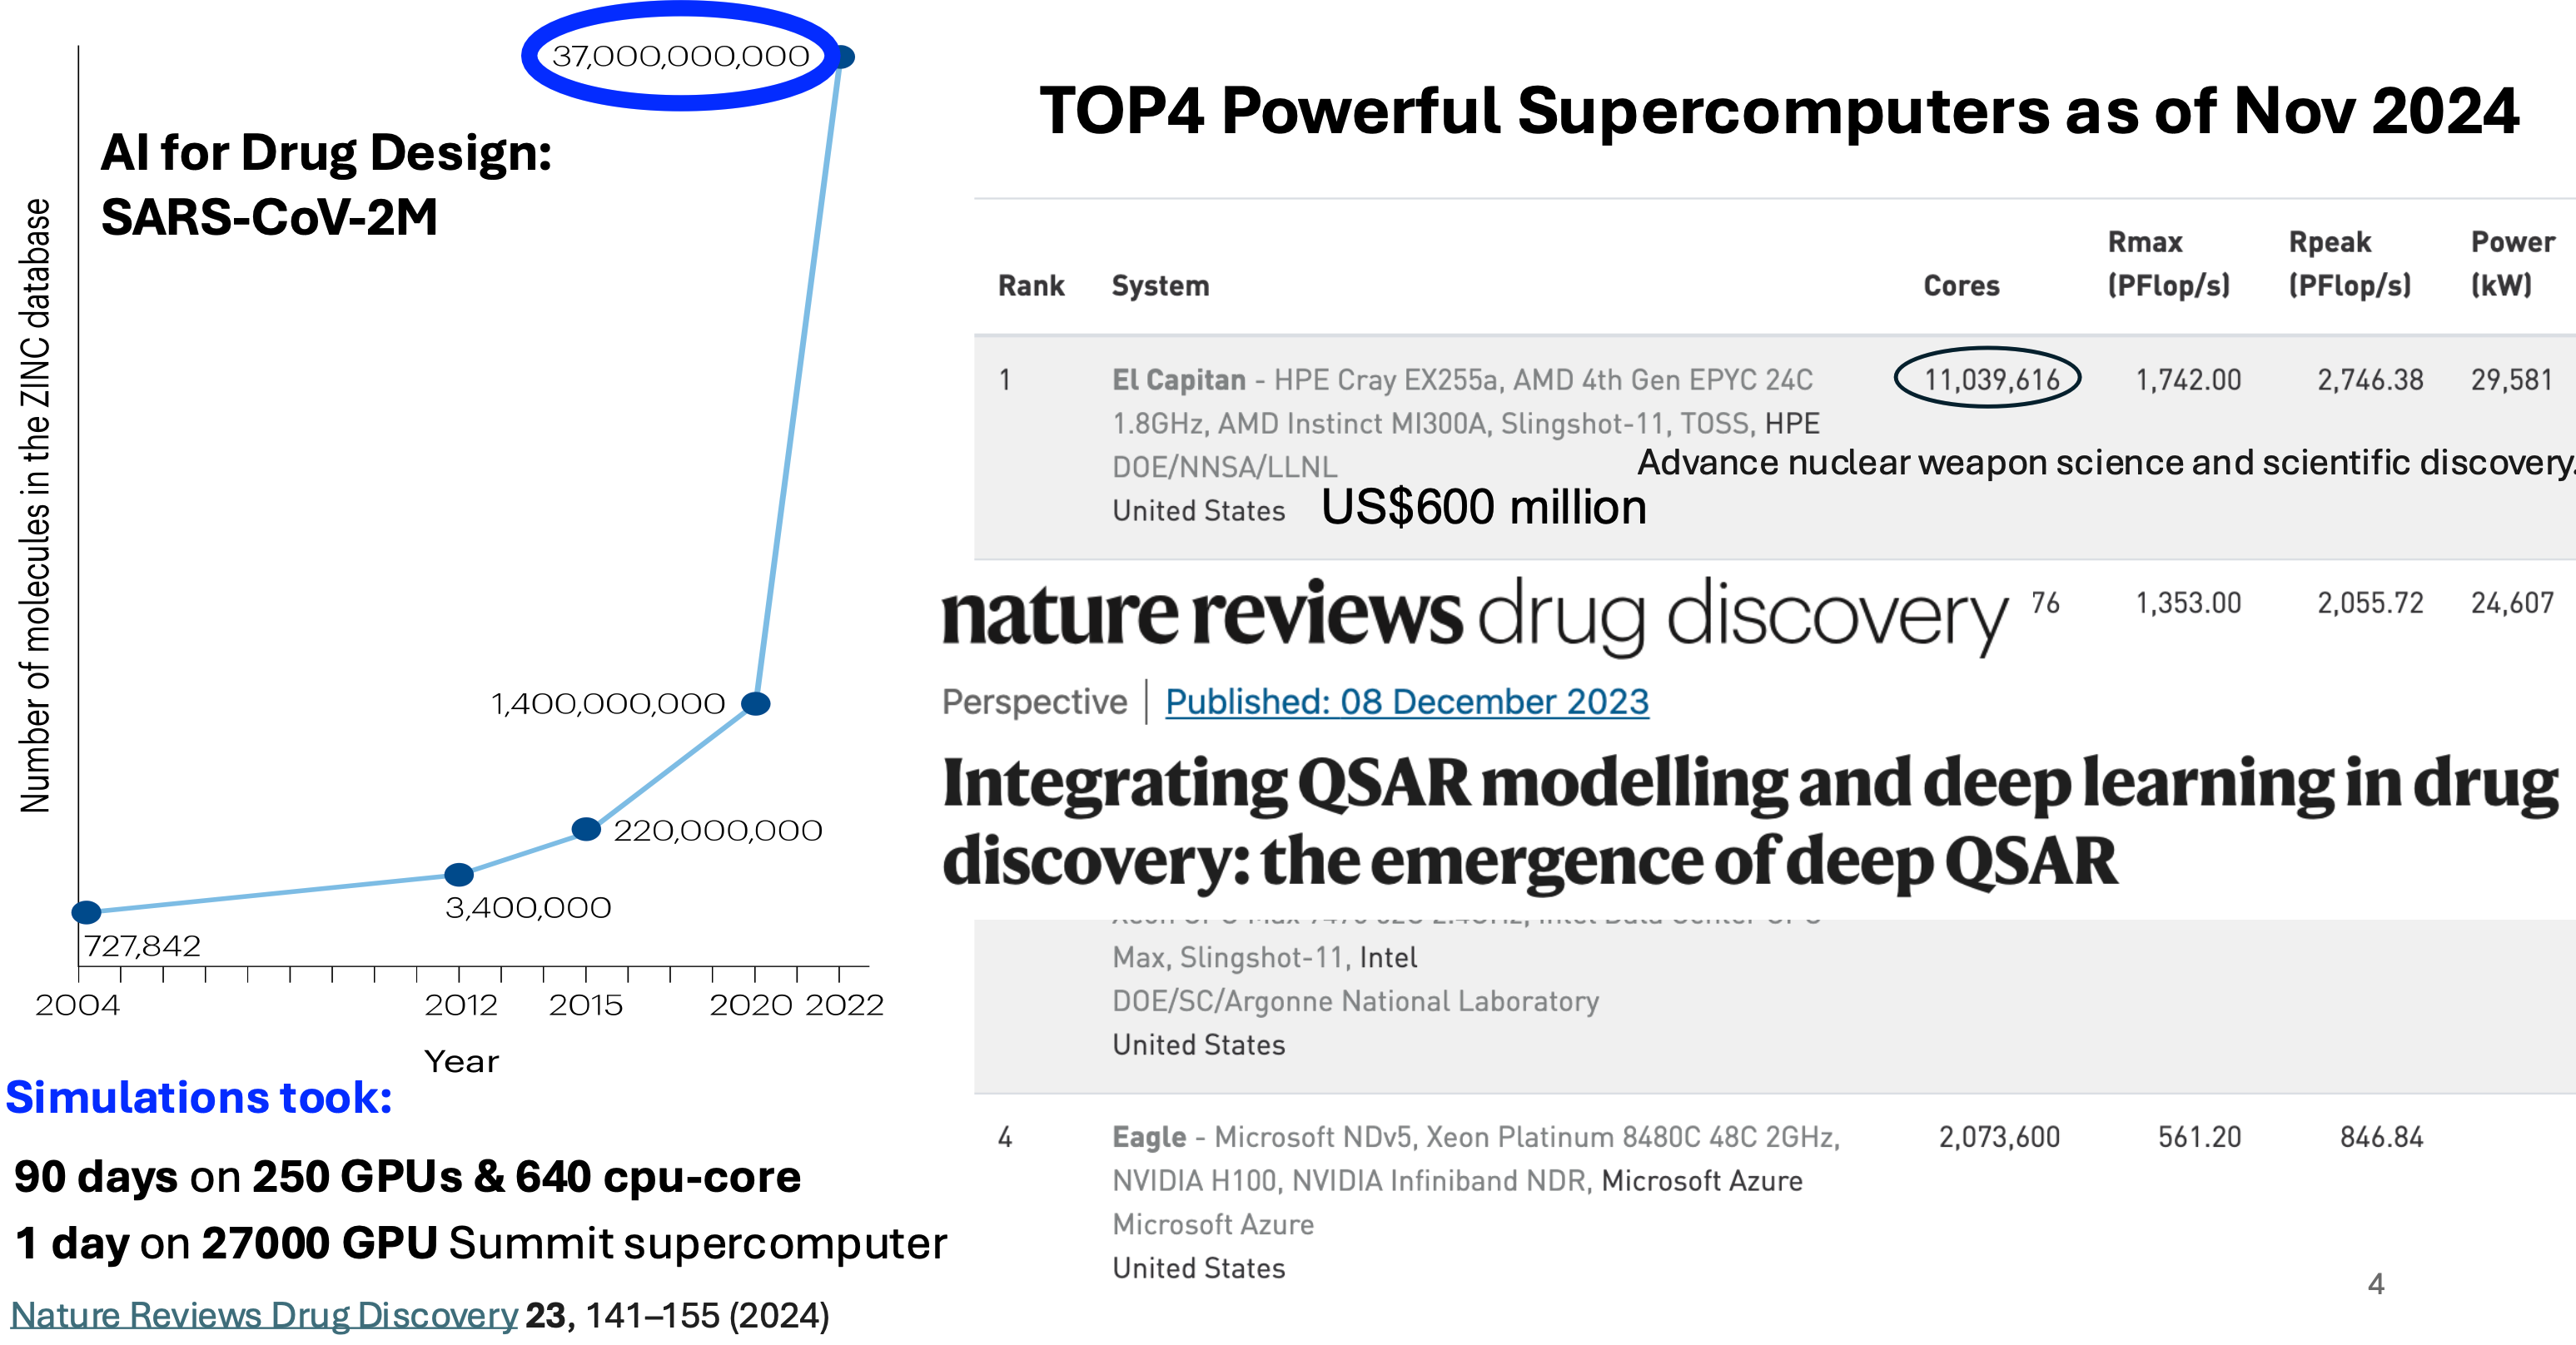
\includegraphics[width=1.0\linewidth]{figures/aitalk2.png}}

\end{frame}


\begin{frame}[plain,fragile]
\frametitle{And power greedy, perhaps quantum computers can reduce the impact?}

% inline figure
\centerline{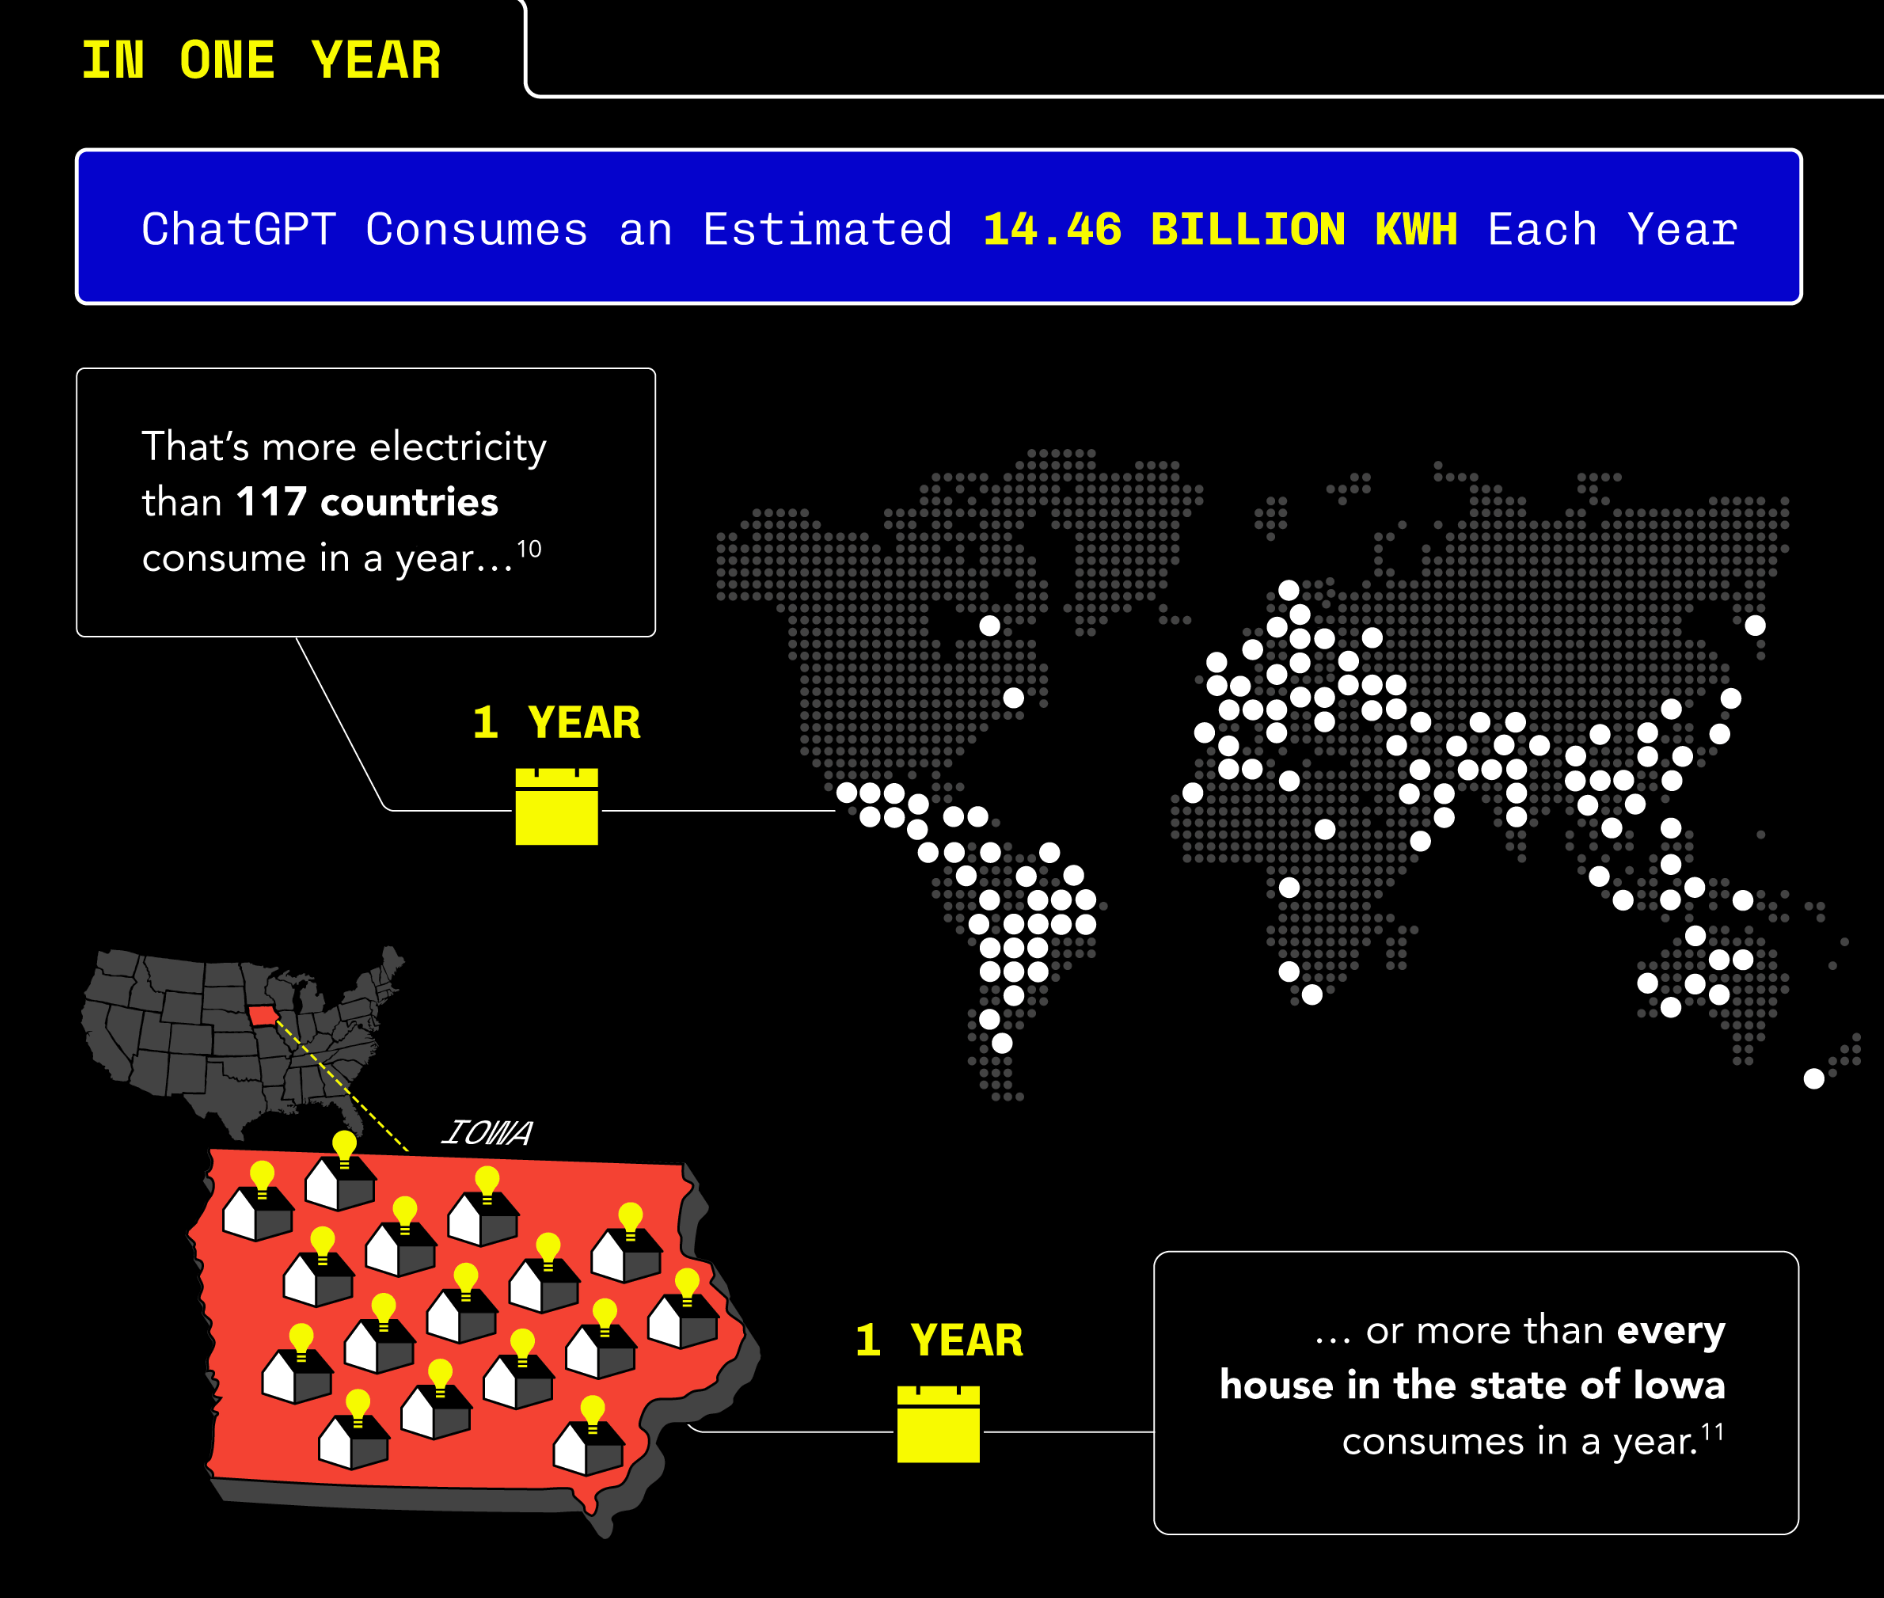
\includegraphics[width=0.7\linewidth]{figures/aitalk1.png}}
Taken from \url{https://www.businessenergyuk.com/knowledge-hub/chatgpt-energy-consumption-visualized/}
\end{frame}





\begin{frame}[plain,fragile]
\frametitle{The plethora  of machine learning algorithms/methods}

\begin{enumerate}
\item Deep learning: Neural Networks (NN), Convolutional NN, Recurrent NN, Boltzmann machines, autoencoders and variational autoencoders  and generative adversarial networks, stable diffusion and many more generative models

\item Bayesian statistics and Bayesian Machine Learning, Bayesian experimental design, Bayesian Regression models, Bayesian neural networks, Gaussian processes and much more

\item Dimensionality reduction (Principal component analysis), Clustering Methods and more

\item Ensemble Methods, Random forests, bagging and voting methods, gradient boosting approaches 

\item Linear and logistic regression, Kernel methods, support vector machines and more

\item Reinforcement Learning; Transfer Learning and more 
\end{enumerate}

\noindent
\end{frame}





\begin{frame}[plain,fragile]
\frametitle{Example of discriminative modeling, \href{{https://www.oreilly.com/library/view/generative-deep-learning/9781098134174/ch01.html}}{taken from Generative Deep Learning by David Foster}}

\vspace{6mm}

% inline figure
\centerline{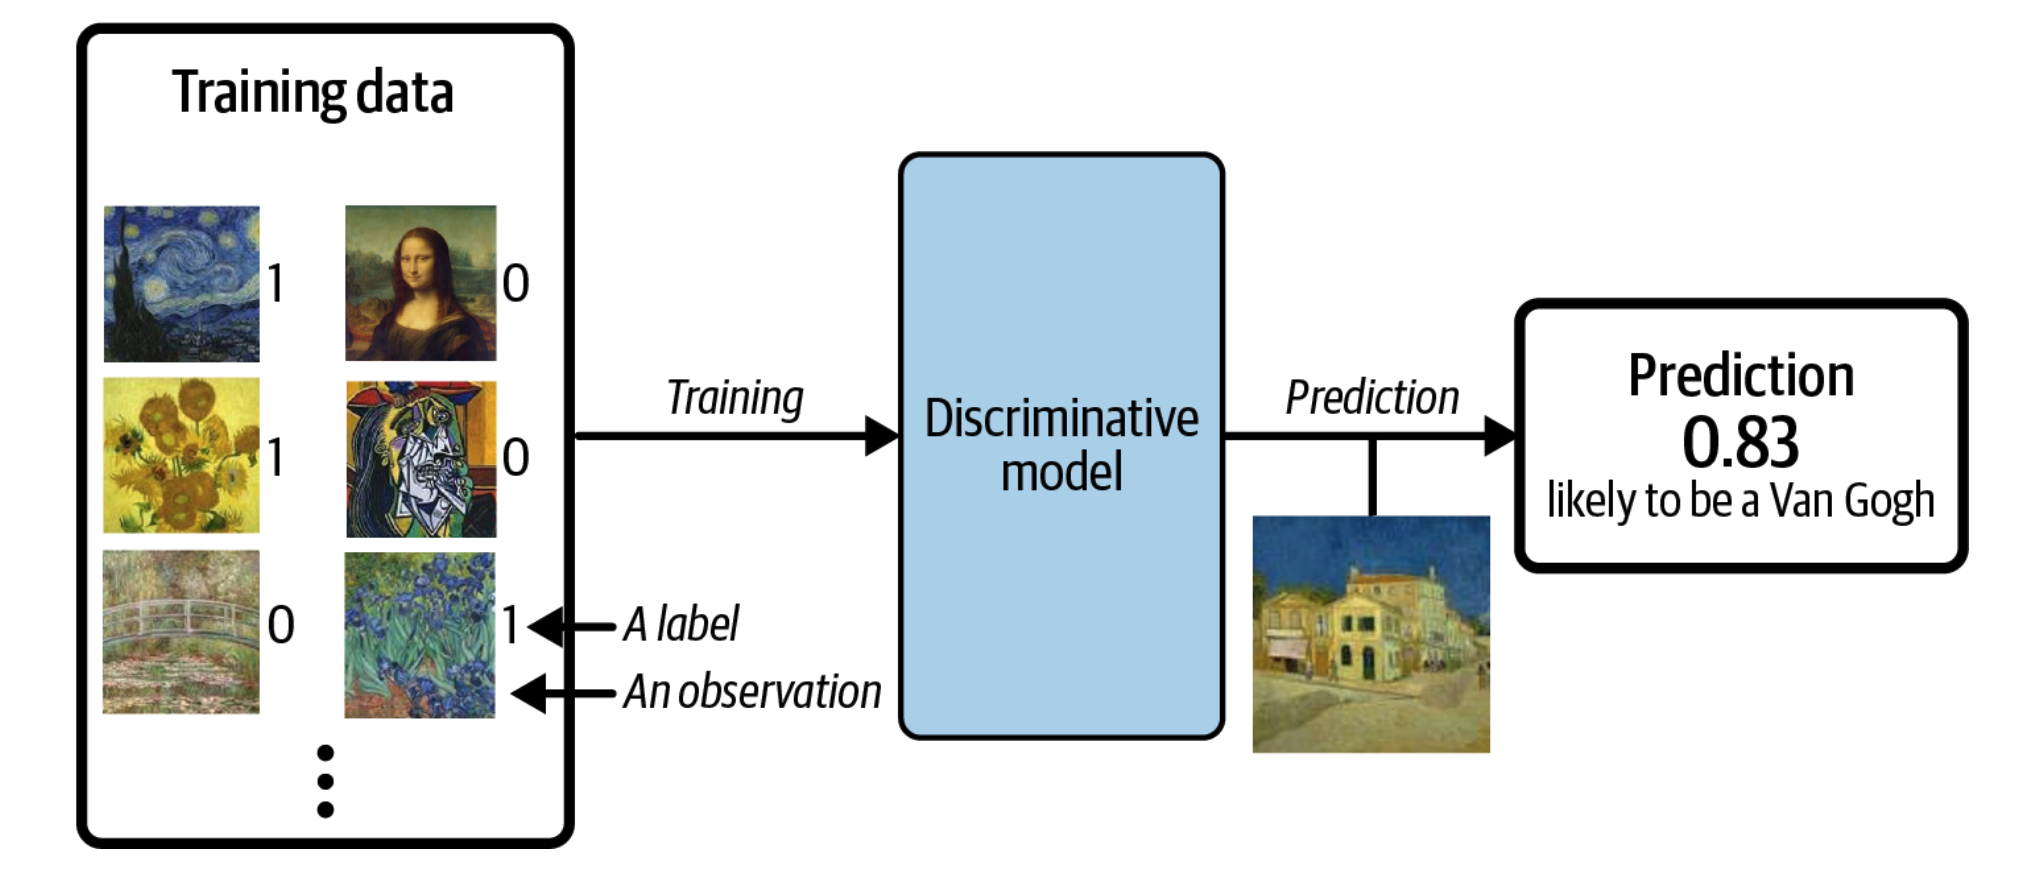
\includegraphics[width=1.0\linewidth]{figures/standarddeeplearning.png}}

\vspace{6mm}
\end{frame}

\begin{frame}[plain,fragile]
\frametitle{Example of generative modeling, \href{{https://www.oreilly.com/library/view/generative-deep-learning/9781098134174/ch01.html}}{taken from Generative Deep Learning by David Foster}}

\vspace{6mm}

% inline figure
\centerline{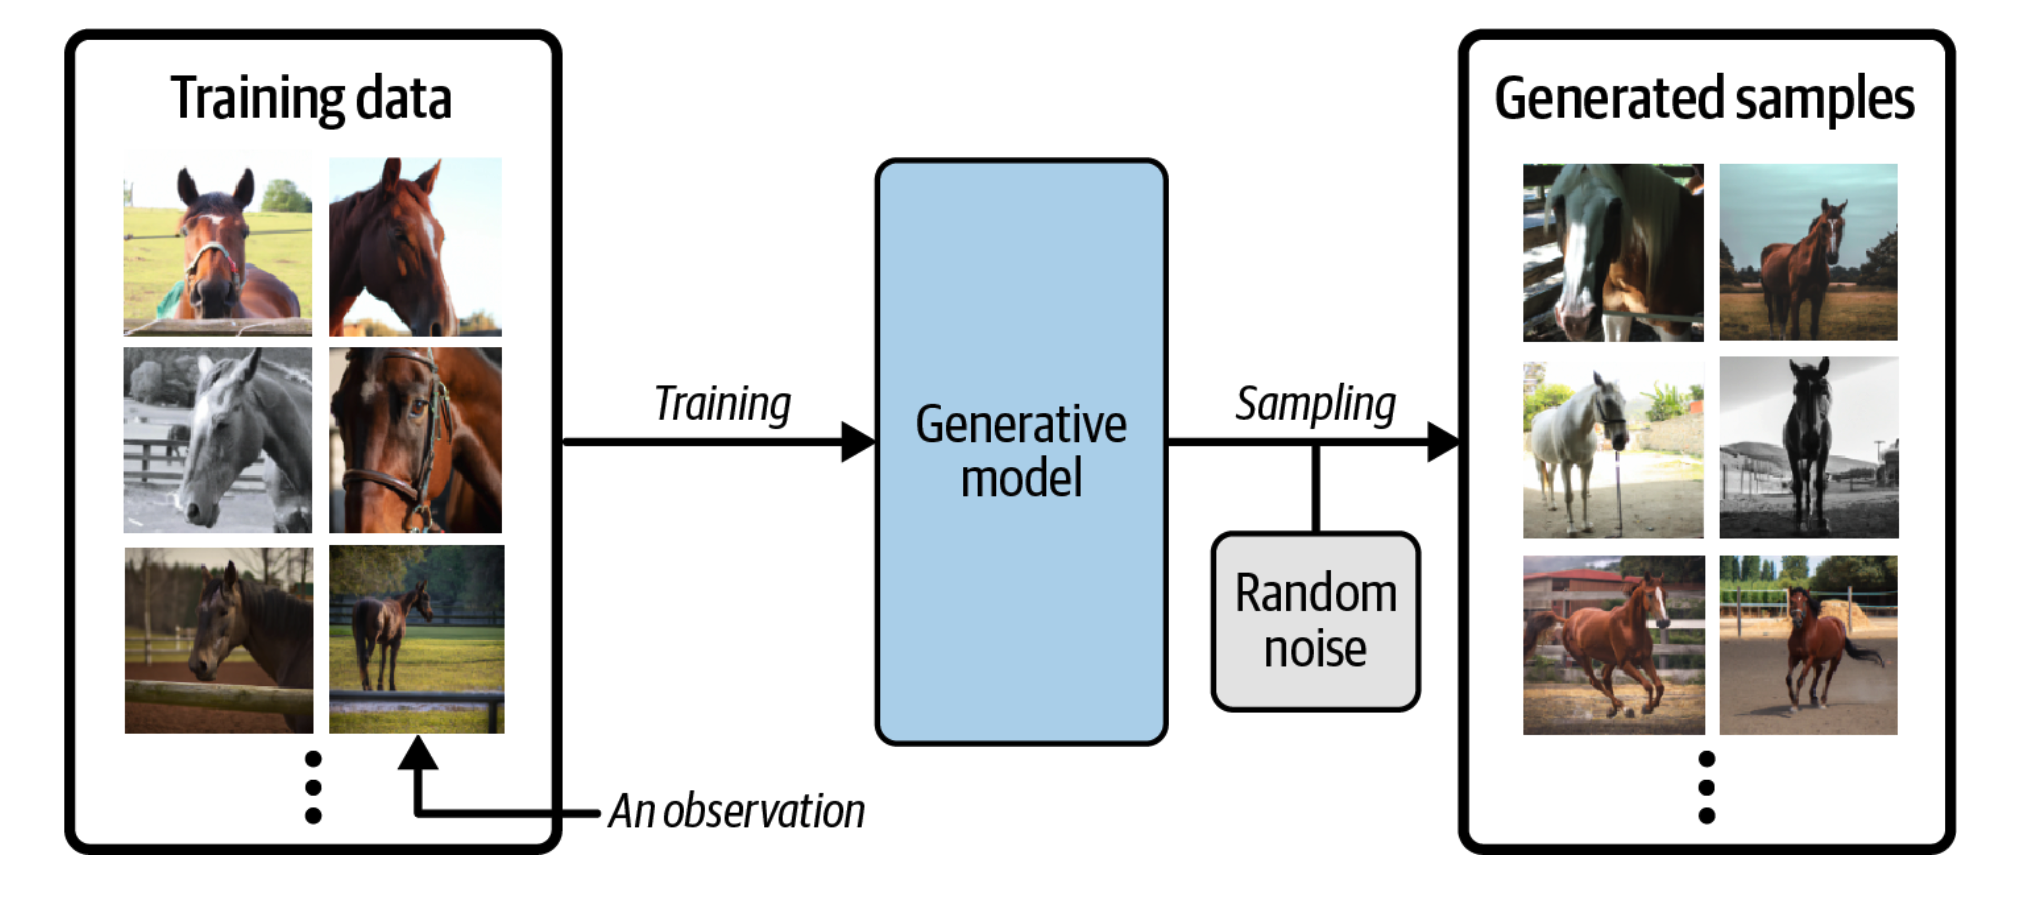
\includegraphics[width=1.0\linewidth]{figures/generativelearning.png}}

\vspace{6mm}
\end{frame}

\begin{frame}[plain,fragile]
\frametitle{Taxonomy of generative deep learning, \href{{https://www.oreilly.com/library/view/generative-deep-learning/9781098134174/ch01.html}}{taken from Generative Deep Learning by David Foster}}

\vspace{6mm}

% inline figure
\centerline{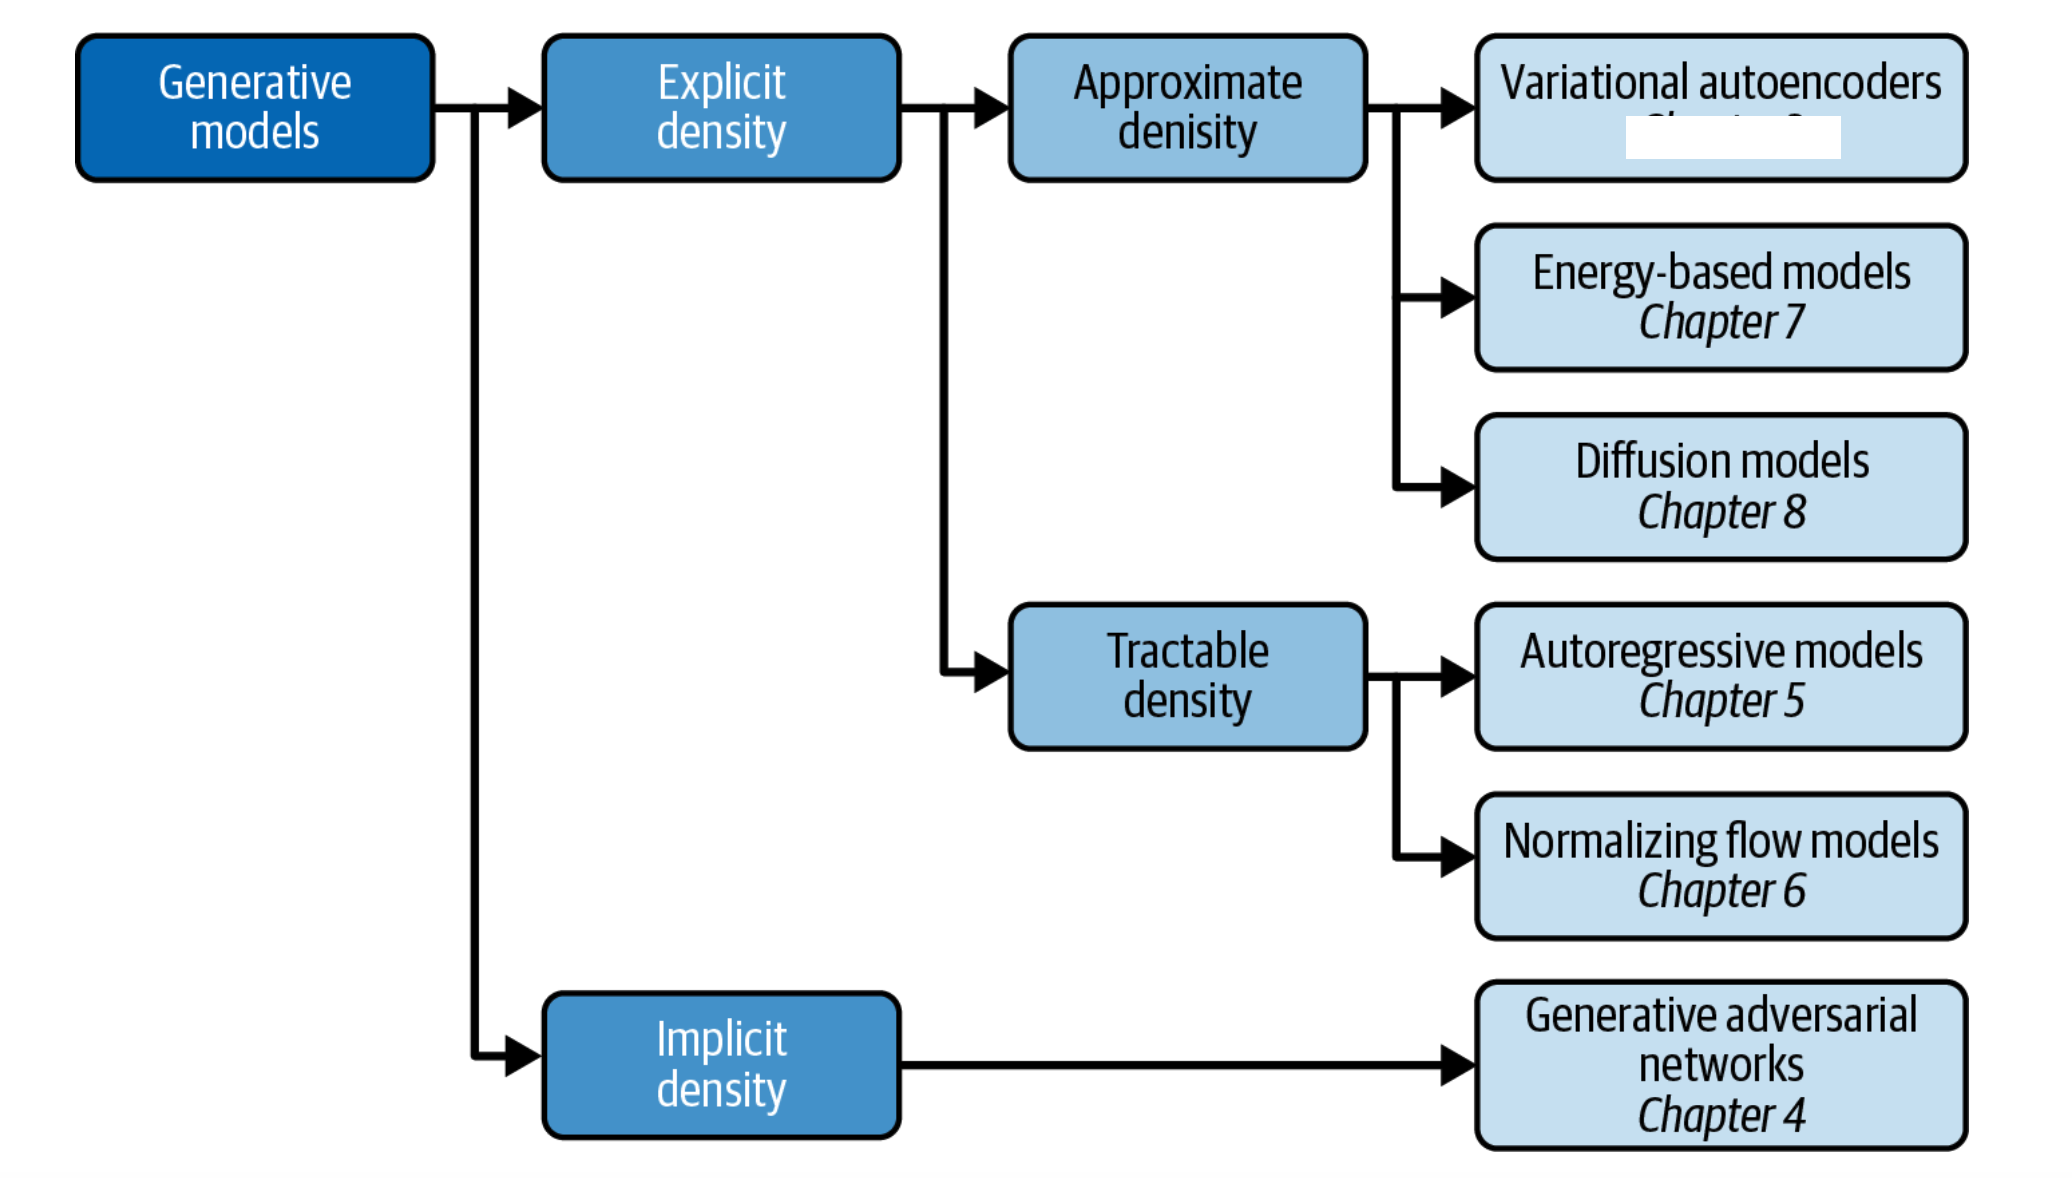
\includegraphics[width=1.0\linewidth]{figures/generativemodels.png}}

\vspace{6mm}
\end{frame}


\begin{frame}[plain,fragile]
\frametitle{What are the basic Machine Learning ingredients?}

\begin{block}{}
Almost every problem in ML and data science starts with the same ingredients:
\begin{itemize}
\item The dataset $\bm{x}$ (could be some observable quantity of the system we are studying)

\item A model which is a function of a set of parameters $\bm{\alpha}$ that relates to the dataset, say a likelihood  function $p(\bm{x}\vert \bm{\alpha})$ or just a simple model $f(\bm{\alpha})$

\item A so-called \textbf{loss/cost/risk} function $\mathcal{C} (\bm{x}, f(\bm{\alpha}))$ which allows us to decide how well our model represents the dataset. 
\end{itemize}

\noindent
We seek to minimize the function $\mathcal{C} (\bm{x}, f(\bm{\alpha}))$ by finding the parameter values which minimize $\mathcal{C}$. This leads to  various minimization algorithms. It may surprise many, but at the heart of all machine learning algortihms there is an optimization problem. 
\end{block}
\end{frame}


\begin{frame}[plain,fragile]
\frametitle{Schematic view on Machine Learning approaches}


% inline figure
\centerline{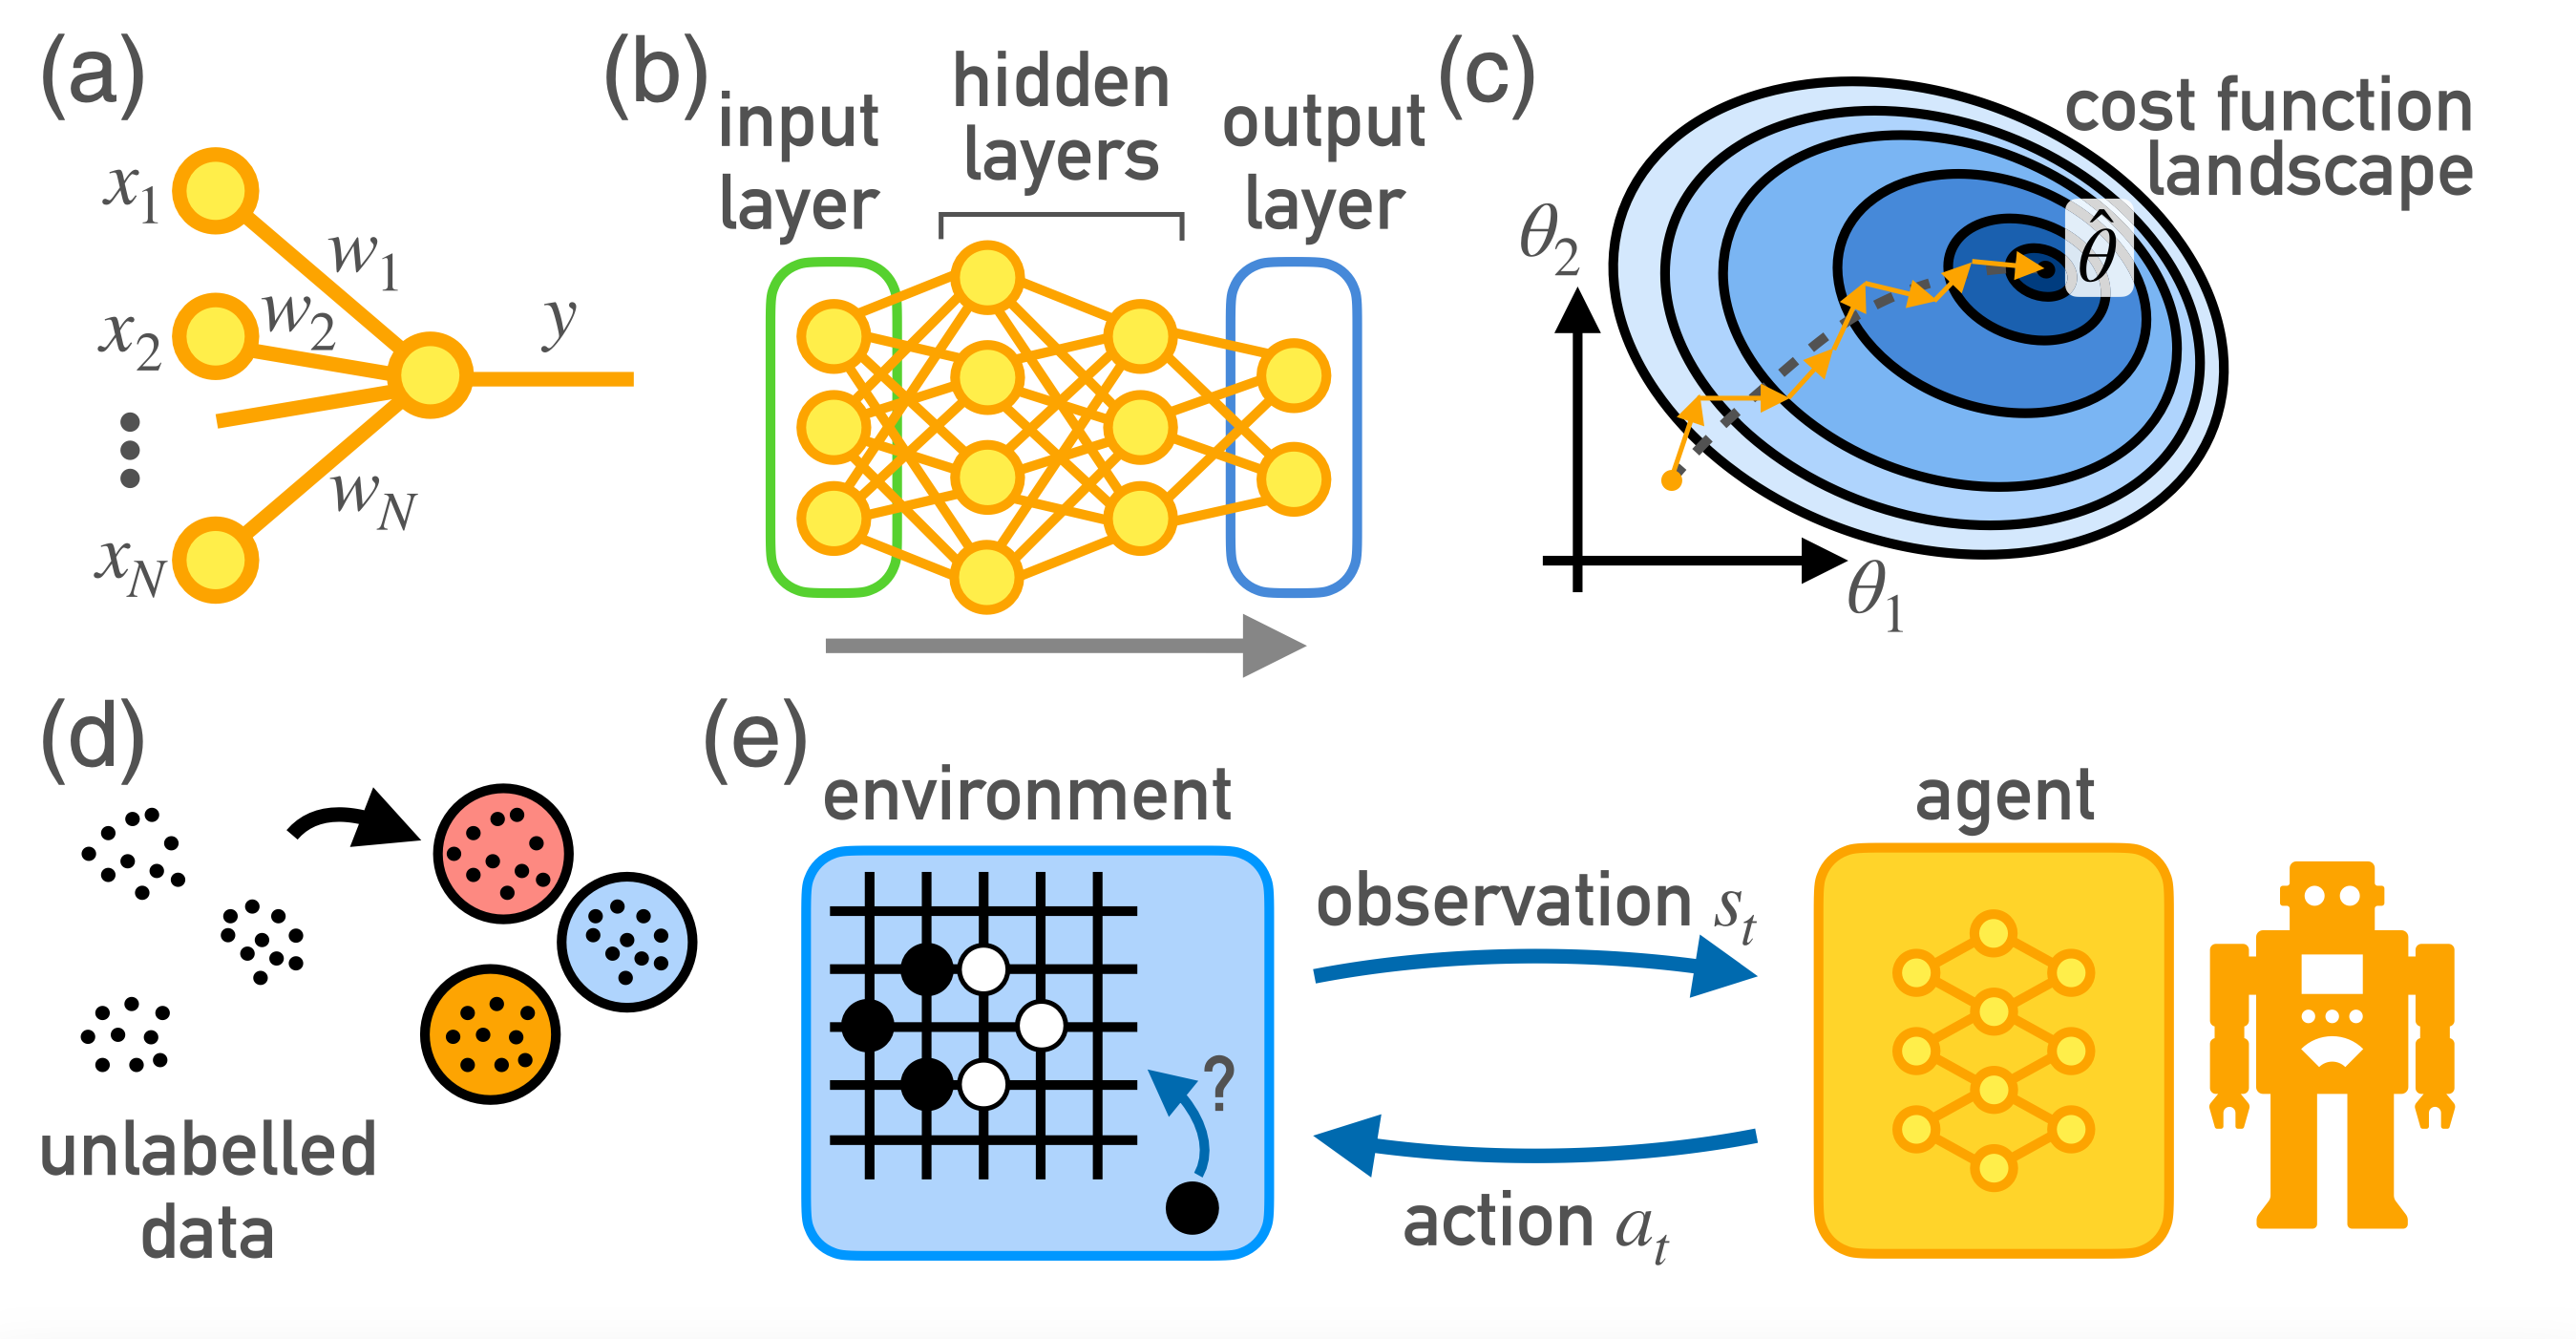
\includegraphics[width=1.05\linewidth]{figures/krenn2}}

\end{frame}


\begin{frame}[plain,fragile]
\frametitle{Quantum technologies and ML/AI}
\centerline{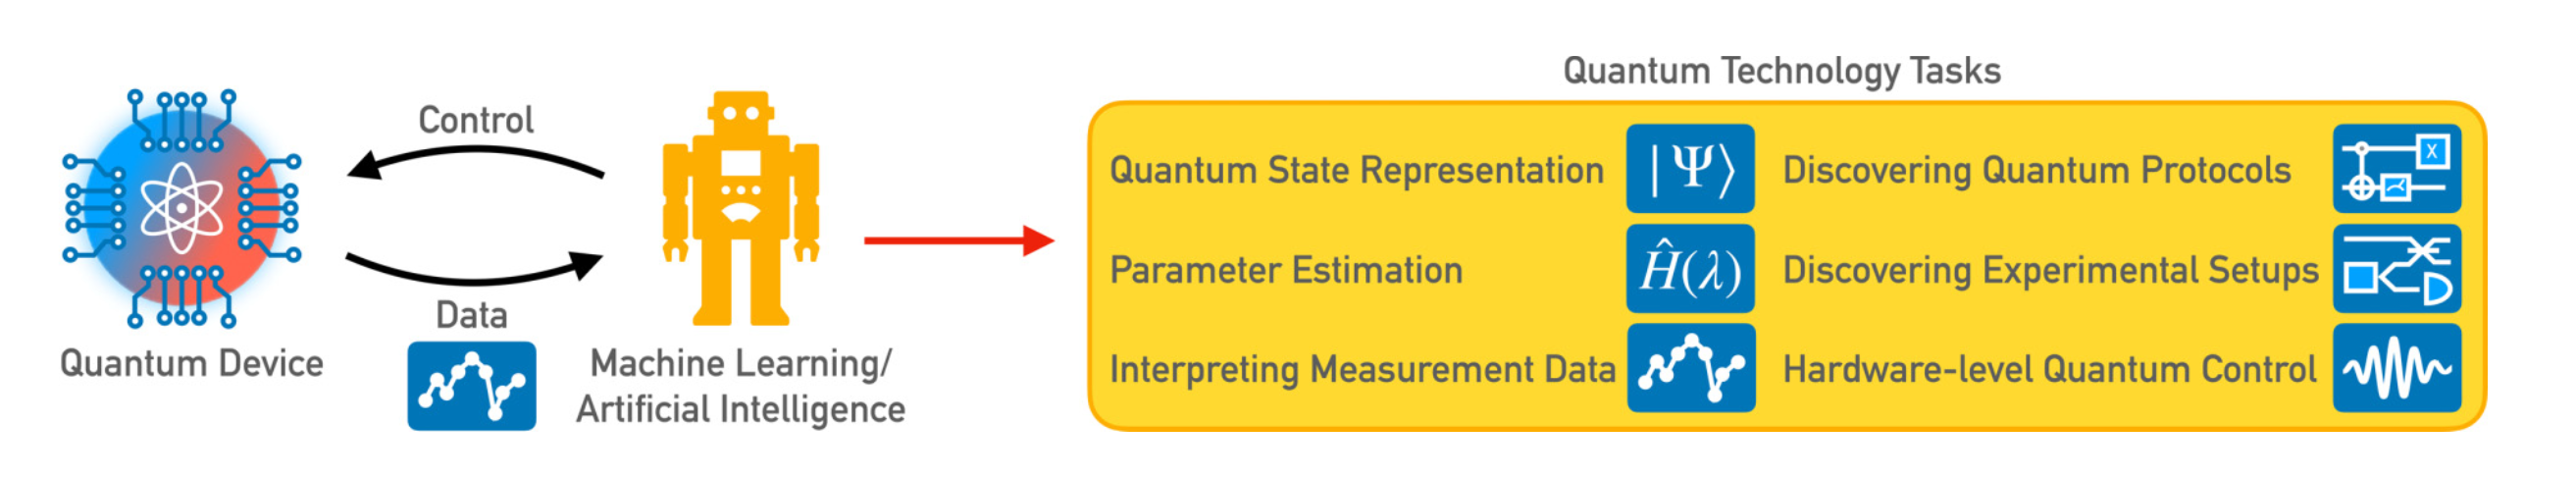
\includegraphics[width=1.05\linewidth]{figures/krenn1}}

\end{frame}


\begin{frame}{What is Quantum Entanglement?}
\textbf{Quantum Entanglement} is a quantum phenomenon where two or more particles become correlated in such a way that the state of one particle directly affects the state of the other, regardless of distance.

\vspace{10pt}
\textbf{Key Features:}
\begin{itemize}
    \item Non-local correlations
    \item No classical analog
    \item Violates Bell's inequalities
\end{itemize}

\textbf{Entangled State Example:}
\[
\ket{\Phi^+} = \frac{1}{\sqrt{2}} (\ket{00} + \ket{11})
\]

\end{frame}


\begin{frame}{1. Quantum Communication}
\textbf{Quantum Teleportation:}
\begin{itemize}
    \item Entanglement enables the transmission of quantum states using classical communication.
    \item No need to send the physical quantum particle.
\end{itemize}

\textbf{Advantage:}
\begin{itemize}
\item Instantaneous state transfer within quantum mechanics constraints.
\item Quantum networks rely on entanglement for secure communication.
  \end{itemize}
\end{frame}

\begin{frame}{2. Quantum Cryptography}
\textbf{Quantum Key Distribution:}
\begin{itemize}
    \item Entanglement ensures secure communication.
    \item Eavesdropping disturbs quantum states, revealing interception attempts.
\end{itemize}

\begin{itemize}
\item Any measurement by a third party collapses the wavefunction.  
\item Ensures security based on quantum mechanics, not computational hardness.
\end{itemize}
\textbf{Advantage:} Unconditional security guaranteed by the laws of physics.
\end{frame}

\begin{frame}{3. Quantum Computing}
\textbf{Speedup in Quantum Algorithms:}
\begin{itemize}
    \item Entanglement provides exponential state space.
    \item Quantum parallelism arises from entangled qubits.
\end{itemize}

\textbf{Grover's Algorithm:}
\[
\mathcal{O}(\sqrt{N}) \text{ vs. } \mathcal{O}(N)
\]

\textbf{Shor's Algorithm:}
\[
\text{Factoring in } \mathcal{O}((\log N)^3)
\]
\end{frame}

\begin{frame}[plain,fragile]
\frametitle{4. Quantum Metrology}

\textbf{Quantum Metrology:}
\begin{itemize}
    \item Uses entangled states for ultra-precise measurements.
    \item Overcomes the classical shot-noise limit.
\end{itemize}

\textbf{Heisenberg Limit:}
\[
\Delta \theta \ge \frac{1}{N},
\]

where \( N \) is the number of entangled particles.  

\begin{block}{Advantage:}
\begin{itemize}
\item Quantum entanglement improves sensitivity beyond classical limits.
\end{itemize}
\end{block}
\end{frame}

\begin{frame}{Challenges of Quantum Entanglement}
\textbf{Decoherence:}
\begin{itemize}
    \item Entangled states are fragile.
    \item Interaction with the environment collapses the wavefunction.
\end{itemize}

\textbf{Scalability:}
\begin{itemize}
    \item Difficult to entangle large numbers of qubits.
    \item Error correction requires complex protocols.
\end{itemize}

\textbf{Measurement Problem:}
\begin{itemize}
    \item Measurement destroys entanglement.
    \item Trade-off between information gain and entanglement preservation.
\end{itemize}
\end{frame}


\begin{frame}[plain,fragile]
\frametitle{Di Vincenzo criteria}

\begin{alertblock}{Quantum computing requirements }
\begin{enumerate}
\item A scalable physical system with well-characterized qubit

\item The ability to initialize the state of the qubits to a simple fiducial state

\item Long relevant Quantum coherence times longer than the gate operation time

\item A \textbf{universal} set of quantum gates

\item A qubit-specific measurement capability
\end{enumerate}

\noindent
\end{alertblock}
\end{frame}


\frame
    {
      \frametitle{Single electrons can make great qubits}
	
      \begin{footnotesize}
     \begin{columns}
       \column{5.0cm}

       At the heart is the trapping and control
       of individual electrons floating above pools of superfluid
       helium. These electrons form the qubits of our quantum
       computer, and the purity of the superfluid helium protects the
       intrinsic quantum properties of each electron. The  ultimate
       goal is to build a large-scale quantum computer based on
       quantum magnetic (spin) state of these trapped electrons.
\column{5cm}
      \begin{center}
	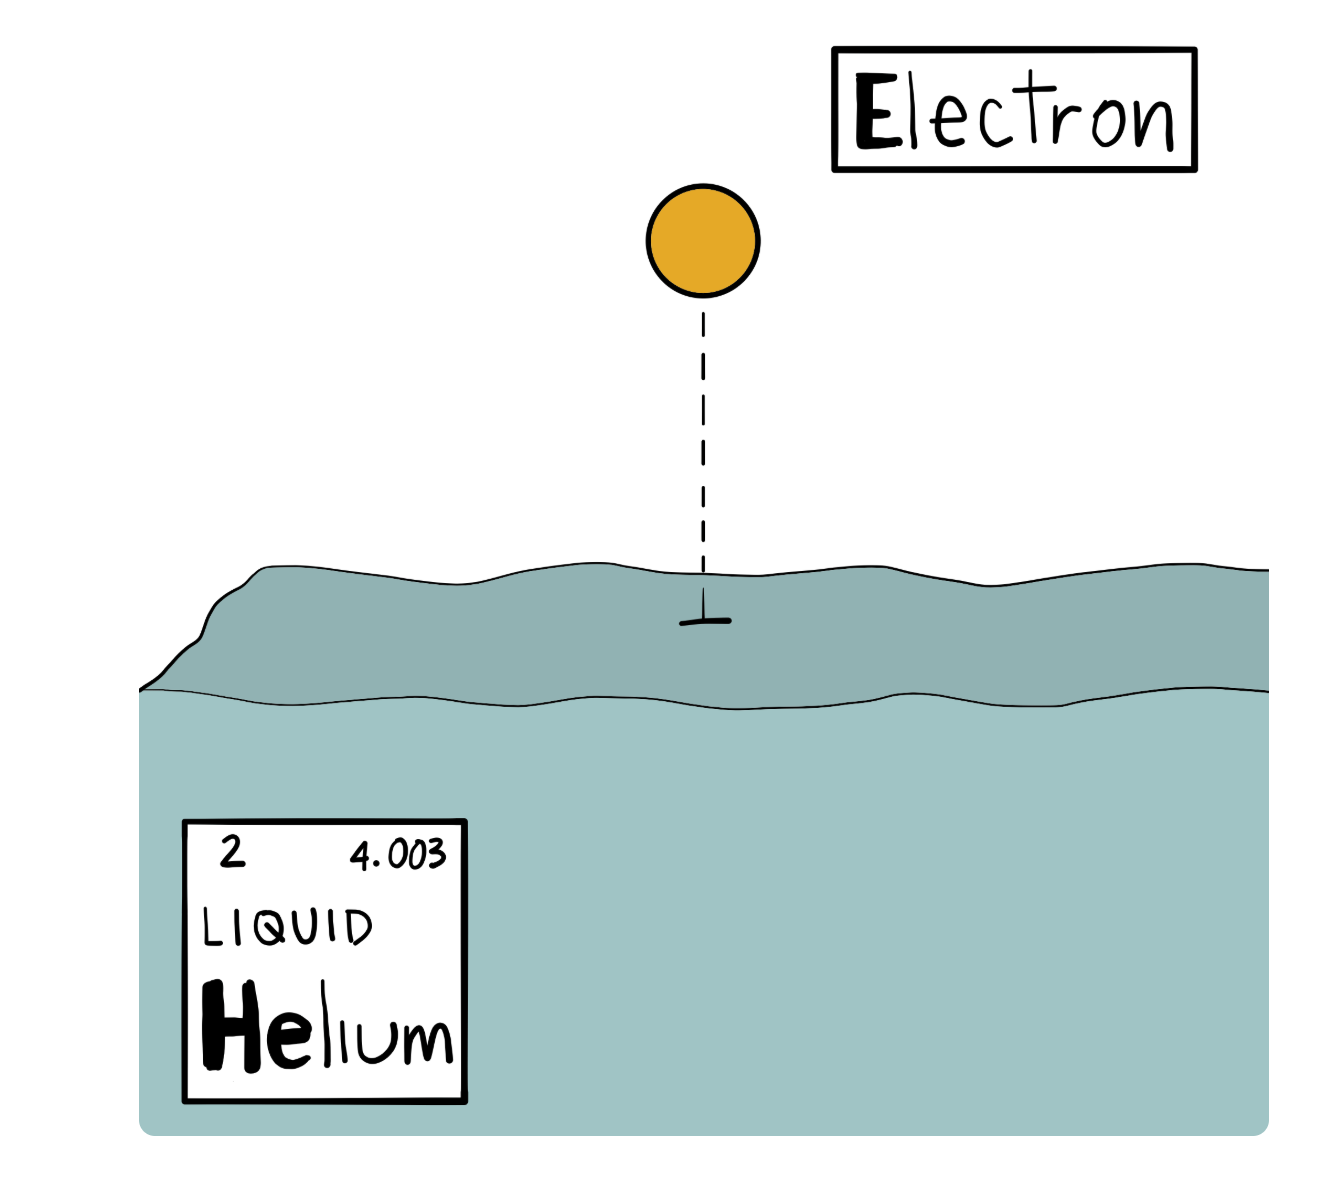
\includegraphics[width=1.2\textwidth]{qcfigures/nordicquantumfig1.png}
      \end{center}
\end{columns}
      \end{footnotesize}
    }


\frame
    {
      \frametitle{Trapping electrons in microchannels}
	
      \begin{footnotesize}
     \begin{columns}
       \column{5.0cm}
Microchannels fabricated into silicon wafers are filled with superfluid helium and energized electrodes. Together with the natural electron trapping properties of superfluid helium, these allow for the precision trapping of individual or multiple electrons. The microchannels are only a few micrometers in size, or about five times smaller than the diameter of a human hair.
\column{5cm}
      \begin{center}
	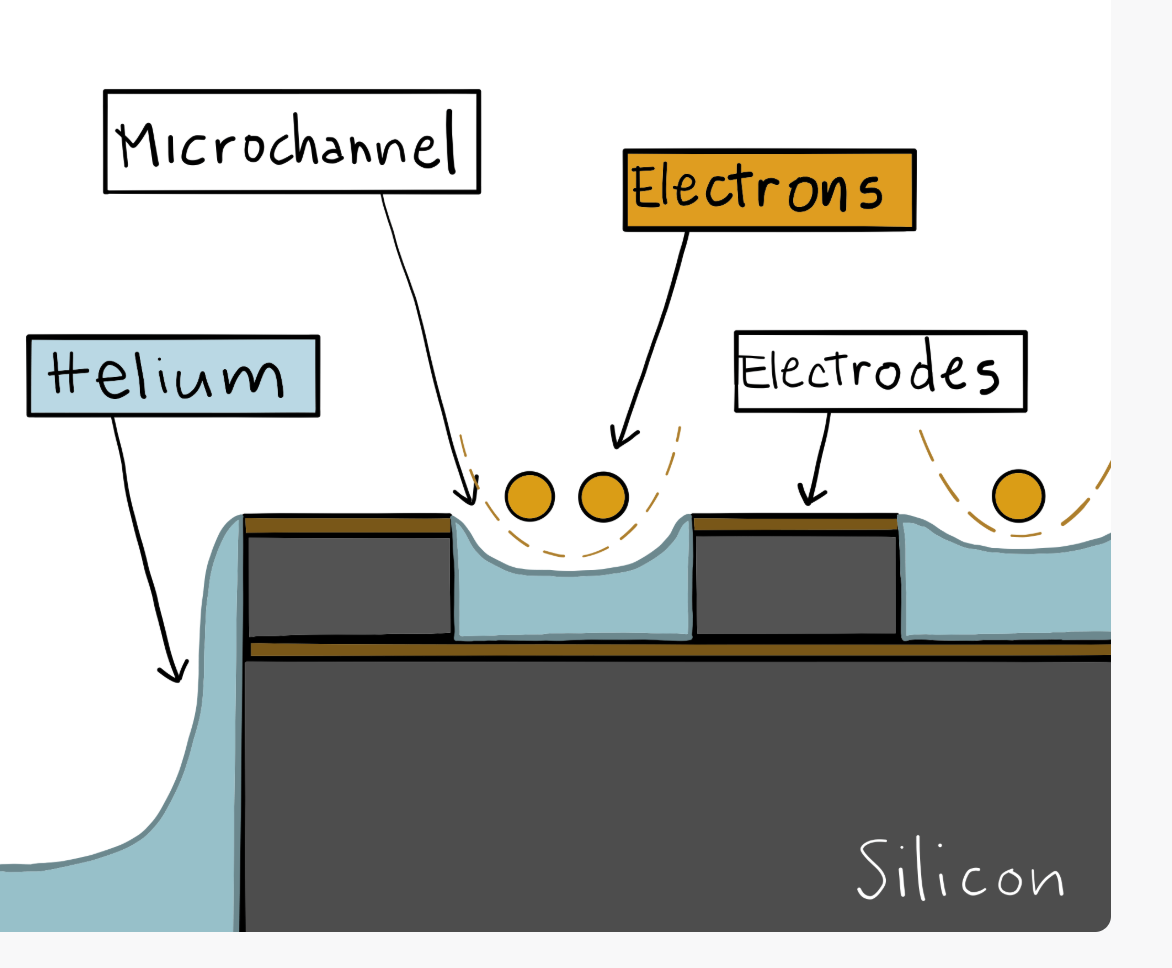
\includegraphics[width=1.2\textwidth]{qcfigures/nordicquantumfig2.png}
      \end{center}
\end{columns}
      \end{footnotesize}
    }

\frame
    {
      \frametitle{Control and readout}
	
      \begin{footnotesize}
     \begin{columns}
       \column{5.0cm}

       Microchannel regions can store thousands of electrons, from which one can be plucked and transported to the single electron control and readout area. In this region, microwave signals will interact with the electron to perform quantum logic gate operations, which will be readout via extremely fast electronics.


\column{5cm}
      \begin{center}
	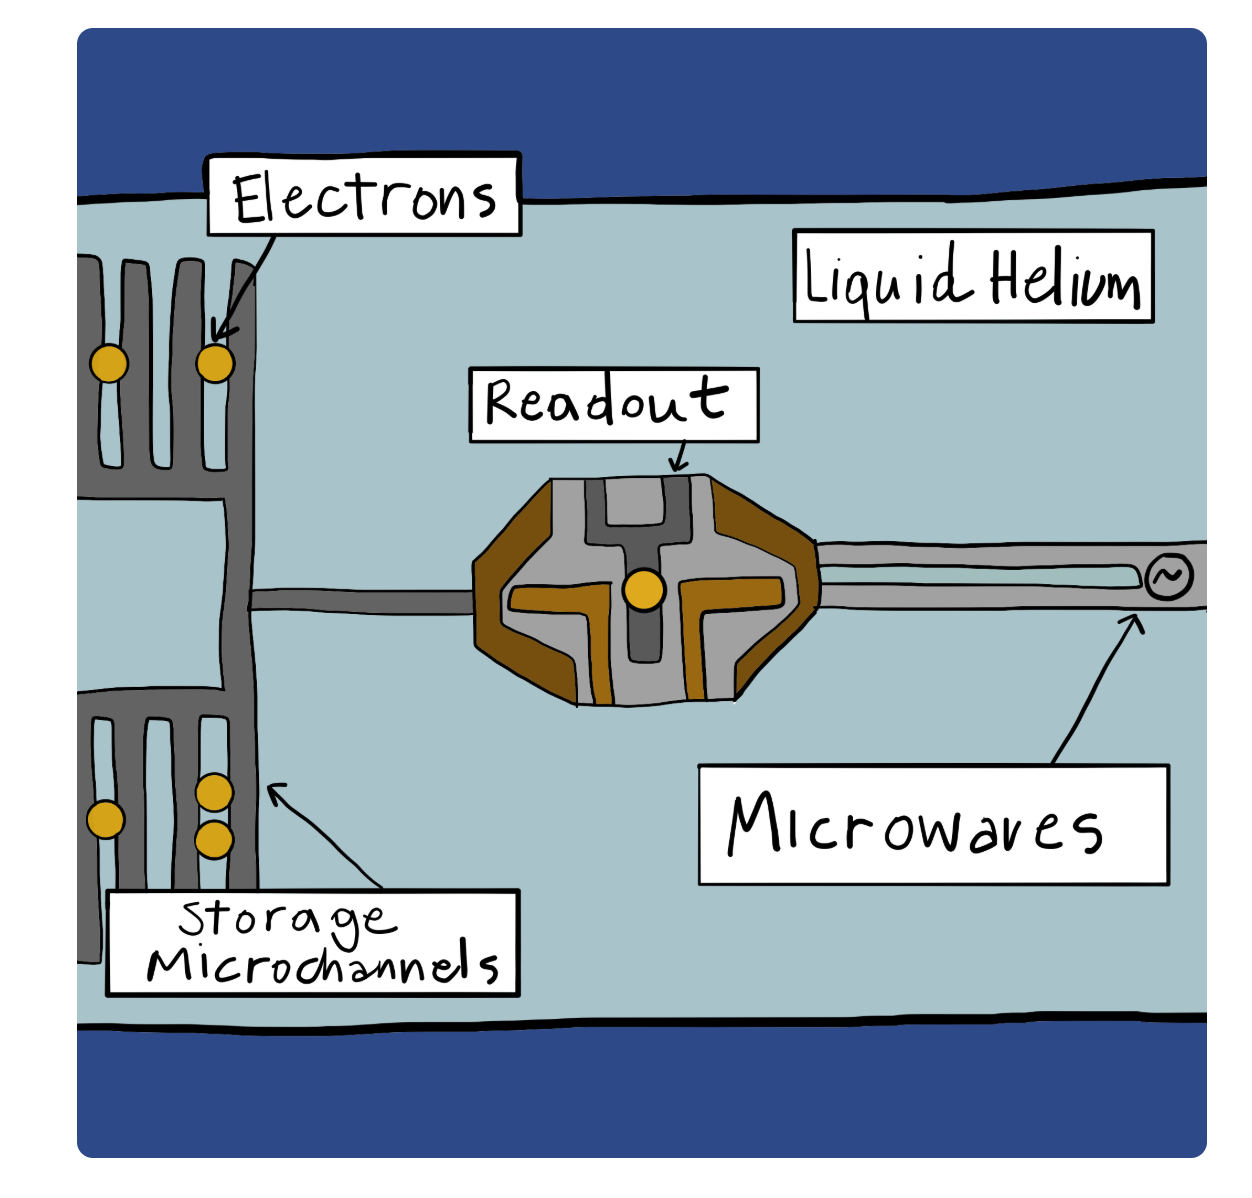
\includegraphics[width=1.2\textwidth]{qcfigures/nordicquantumfig3.png}
      \end{center}
\end{columns}
      \end{footnotesize}
    }


\frame
    {
      \frametitle{Operations for quantum computing}
	
      \begin{footnotesize}
     \begin{columns}
       \column{5.0cm}
Quantum information can be encoded in a number of ways using single electrons. Currently, we are working with the side-to-side(lateral) quantum motion of the electron in the engineered trap. This motion can either be in its lowest energy state, the ground state, or in a number of higher-energy excited states. This electron motion also provides the readout capabilities for the ultimate goal of building a large-scale quantum computer based on the electron's magnetic moment (spin).       
\column{5cm}
      \begin{center}
	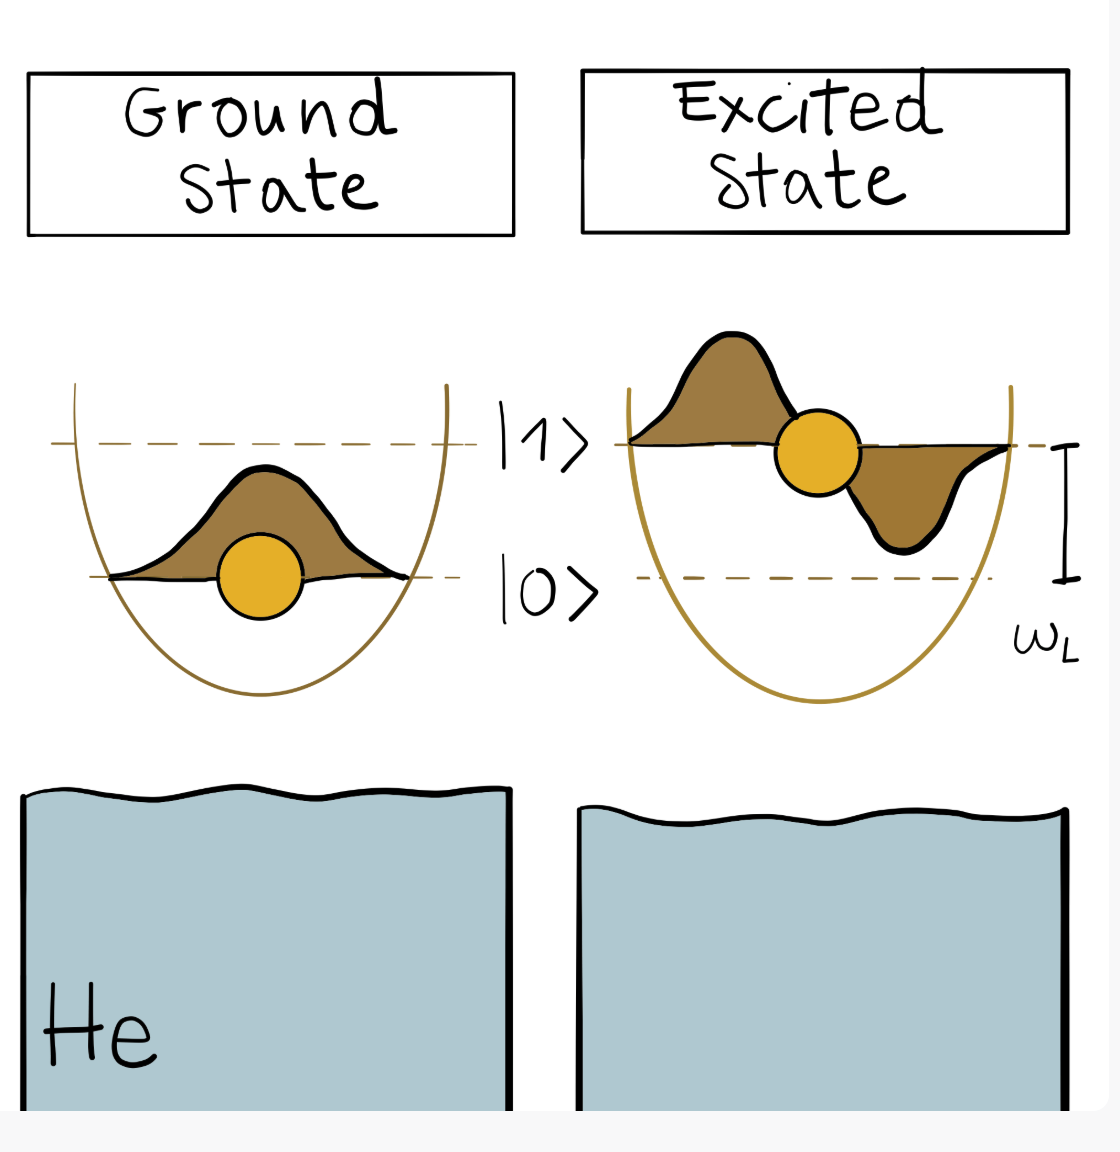
\includegraphics[width=1.2\textwidth]{qcfigures/nordicquantumfig4.png}
      \end{center}
\end{columns}
      \end{footnotesize}
    }
    





\begin{frame}[plain,fragile]
\frametitle{Can I study these topics at UiO?}


\begin{itemize}
\item Several courses on Machine learning and AI at UiO, from bachelor level to PhD level, see \url{https://github.com/CompPhysics/MachineLearning}
\item Quantum technologies, quantum information theory, quantum computing, quantum sensing and more. Study directions in Physics bachelor degree, Physics master degree and Computational Science master of science program
  \begin{enumerate}
  \item Physics Bachelor of Science program  \url{https://www.uio.no/studier/program/fysikk-astronomi/studieretninger/kvanteteknologi/index.html}
  \item Physics Master of Science program \url{https://www.uio.no/english/studies/programmes/physics-master/programme-options/quantum-technology/index.html}
  \item Computational Science Master of Science program \url{https://www.uio.no/english/studies/programmes/computational-science-master/programme-options/quantum-technology/index.html}
    \end{enumerate}
\end{itemize}

\end{frame}


\end{document}






